\documentclass[11pt,a4paper]{article}

%include polycode.fmt

\usepackage[margin=2.5cm]{geometry}
\usepackage{todonotes}
\usepackage{microtype}
\usepackage{amssymb,amsmath}
\usepackage{mathpazo}
\usepackage{accents}
\usepackage{longtable,booktabs}
\usepackage{dcolumn}
\usepackage{pgf}
\usetikzlibrary{shapes.geometric}
\usetikzlibrary{matrix}
\usepackage{natbib}
\usepackage{hyperref}
\usepackage[capitalise,noabbrev,nameinlink]{cleveref}
\hypersetup{
  pdftitle={Storing the Cardano ledger state on disk: API design concepts},
  pdfborder={0 0 0},
  breaklinks=true
}

\DeclareMathOperator{\dom}{dom}
\newcommand\restrict[2]{\left.#1\right|_{#2}}
\newcommand\deltavar[1]{\accentset{\Delta}{#1}}
\newcommand\eqabove[2]{\begin{array}{c}#1\\=\\#2\end{array}}

\begin{document}

\title{Storing the Cardano ledger state on disk: \\
       API design concepts \\
       {\large \sc An IOHK technical report}
  }
\date{Version 0.6, August 2023}
\author{Duncan Coutts      \\ {\small \texttt{duncan@well-typed.com}} \\
                              {\small \texttt{duncan.coutts@iohk.io}} \\
   \and Douglas Wilson     \\ {\small \texttt{douglas@well-typed.com}} \\
   \and Joris Dral         \\ {\small \texttt{joris@well-typed.com}} \\
                              {\small \texttt{joris.dral@iohk.io}} \\
   }

\maketitle

\section{Purpose}

This document is intended to explore and communicate -- to a technical audience
-- design concepts for how to store the bulk of the Cardano ledger state on
disk, within the context of the existing designs of the Cardano consensus and
ledger layers. We will try to illustrate the ideas with prose, algebra,
diagrams, and models.

The reader is assumed to be familiar with the initial report on this topic,
covering analysis and design options \citep{utxo-db}.

\section{Acknowledgements}

Thanks to the consensus team for many useful discussions and feedback. Thanks
particularly to Edsko de Vries for critiques of early versions of these ideas.
Thanks to Tim Sheard for the inspiration to use the ideas and notation of a
calculus of changes.

\tableofcontents

\section{Ledger state handling in the current design}
\label{ledger-state-handling-in-the-current-design}

\subsection{In the ledger layer}
\label{ledger-state-handling-in-the-current-ledger-layer}

The existing ledger layer relies heavily on using pure functions to manipulate
and make use of the ledger state. In particular, the ledger rules are written in
a style where old and new states are passed around explicitly. The ledger rules
are complex and non-trivial to test, so the benefits of using a pure style are
substantial and not something that we would wish to sacrifice.

\subsection{In the consensus layer}
\label{ledger-state-handling-in-the-current-consensus-layer}

The consensus layer relies on the ledger layer for the functions to manipulate
the ledger state, but the design of the consensus layer relies on these
functions being pure.

The consensus layer also relies on the use of in-memory,
persistent\footnote{That is persistent in the sense of purely functional data
structures, not persistent as in kept on disk} data structures. It keeps the
ledger states for the last $k$ blocks of the chain in memory. The consensus
layer also evaluates speculative ledger states along candidate chains, which may
be adopted or discarded. Overall, there is not just a single logical ledger
state in use at once -- there are many related ones. There are enormous
opportunities for sharing between these related ledger states and the use of
persistent data structures takes full advantage, such that the cost is little
more than the cost of a single ledger state. The incremental cost is
proportional to the \emph{differences} between the states.

Having quick and easy access to the ledger states of the last $k$ blocks is not
a design accident. An important design principle for the Cardano node has been
to balance the resource use in all interactions between honest nodes and
potentially dishonest nodes and thus resist DoS attacks. This design principle
led us to an Ouroboros design that involves efficient access to recent ledger
states. \citet{fake-stake} describe the consequences of the failure to adopt
this design principle. They identify a pair of flaws in the design of many
other PoS blockchain implementations which lead to resource imbalances that can
be exploited to mount DoS attacks. This was reported in the popular press as
the so-called `fake stake attack'%
\footnote{For example \url{https://www.zdnet.com/article/security-flaws-found-in-26-low-end-cryptocurrencies/}}.
One of the design flaws involves not having efficient access to recent ledger
states and consequently postponing block body validation to the last possible
moment.

In our design to store much of the ledger state on disk, it is essential that we
preserve the ability to efficiently access and use the ledger states for the
last $k$ blocks. Our resistance to DoS attacks depends on it.

Furthermore, chain selection within consensus relies on the ability to evaluate
the validity of candidate chains without yet committing to them. This also
relies on being able to compute derived ledger states

\section{Terminology and our perspective on databases}
\label{terminology}

We will make use of the terminology of databases as well as Cardano blockchain
terminology. This is potentially confusing since transactions are an important
concept in both databases and blockchain ledgers.

In this document we will mostly talk about transactions in the database sense.
As it turns out, the processing of transactions in the database sense
(usually\footnote{For chain validation, the database transactions are the ledger
state transformations arising from applying blocks to a chain. For mempool
validation, the database transactions are the ledger state transformations
arising from new blockchain transactions being added to the mempool.})
corresponds to processing of whole blocks in the blockchain.

We will take a relatively abstract view of databases. For the most part, we will
consider databases simply as logical values without any particular implication
of a choice of representation. Where it is important to imagine that a
representation would be in-memory or on-disk, we will try to be clear about
it. In this same spirit, we will talk (and reason) about multiple logical
values of a database, even though real databases typically only allow access
to the `current' value of the database. In this abstract view of databases, a
transaction is simply a way to get from one logical value of the database to
another.

This is exactly the same mathematical perspective we take with functional
programming: new values are defined based on old values. It is also exactly how
we define our ledger rules as functions on the ledger state: given an old state,
it yields an updated state (with the old one still available). A database
perspective on the blockchain ledger would say that the ledger state itself is
the database and that the transactions on that database are the ledger state
transformations arising from extending the chain with additional blocks. This is
the perspective we will take.

\section{General approach}
\label{general-approach}

We wish to deviate as little as possible from the general design of the current
ledger and consensus layers, particularly with respect to using pure functions
and persistent data structures.

The ledger state will be maintained using a partitioned approach with both
in-memory and on-disk storage. The large key-value mappings will be kept primarily on
disk, and all other state will be kept in memory.

We will manipulate the state using pure functions over immutable, in-memory data
structures. This relies on two main ideas: reading the data into memory in
advance, and working with differences of data structures.

\subsection{Inspiration from the `anti-caching' database architecture}
\label{anti-caching}

Our general approach takes inspiration from \citet{anti-caching} who describe an
OLTP\footnote{OLTP stands for Online Transaction Processing, which is a style of
database workload. A blockchain ledger database would be subjected to such a
workload.} database architecture that they call `anti-caching'.

The anti-caching architecture reverses the usual notion that a database's value
is represented on disk while some data is cached in memory for efficiency.
Instead, the perspective is that the logical value of the database is
represented in memory while much of the data is evicted from memory to disk.
This is the essence of the eponymous anti-cache: the disk is used as an
anti-cache to evict in-memory data, rather than using memory as a cache for disk
data.

%\begin{figure}[h]
\begin{center}
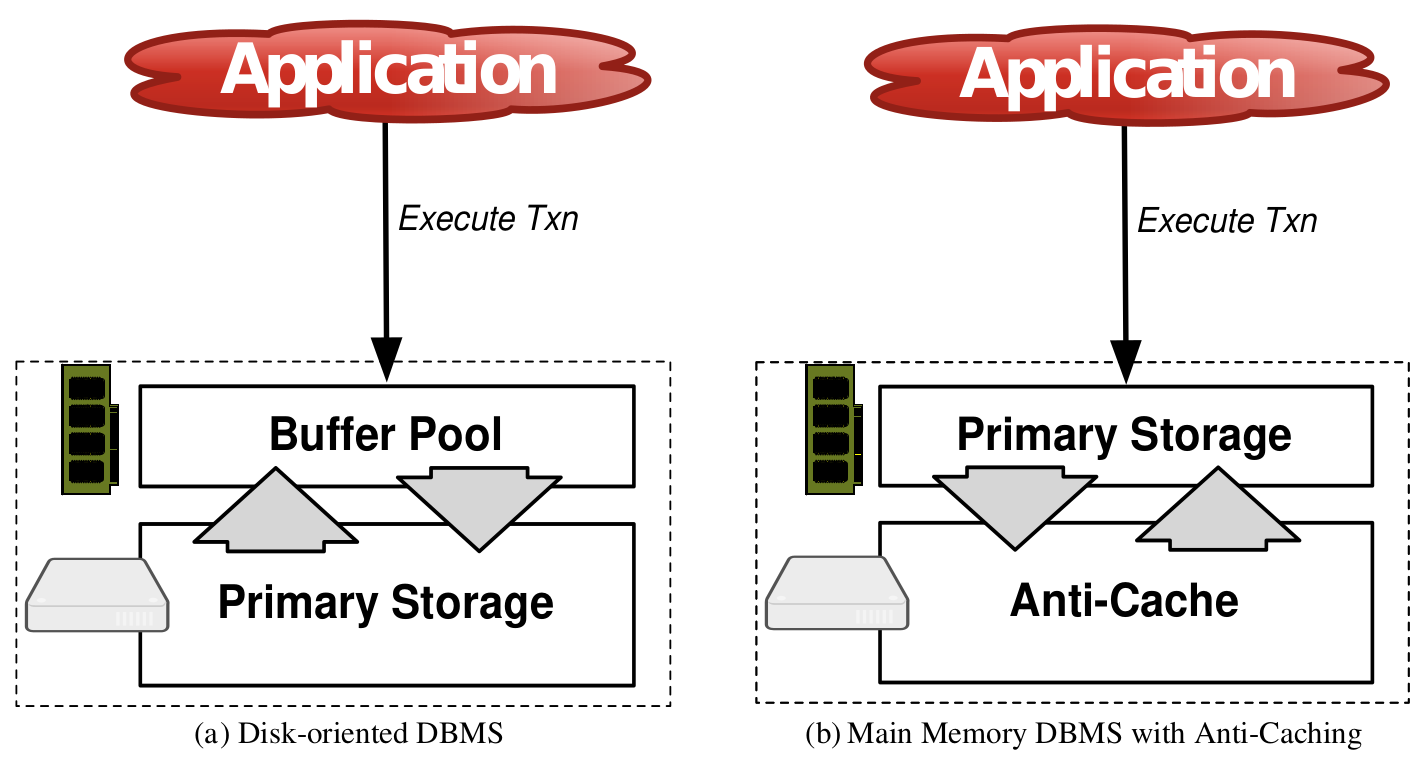
\includegraphics[scale=0.25]{img/hstore-anticaching-fig1.png}
\begin{quote}
Diagram by \citet[Figure 1]{anti-caching} illustrating the difference in
database architecture: ``In (a), the disk is the primary storage for the
database and data is brought into main memory as it is needed. With the
anti-caching model in (b), memory is the primary storage and cold data is
evicted to disk.''
\end{quote}
\end{center}
%\end{figure}

One of the ideas we borrow is that the logical value of the database is
determined by the in-memory data, with large parts of the data residing on-disk.
This means that, as a matter of principle, we do not need to constrain ourselves
to keeping all data on disk. We merely need to keep most of it on disk. Where
there are efficiency or design complexity benefits, we can choose to keep data
in memory, provided that we do not exhaust our overall memory budget.

Another feature of the anti-caching architecture is that all data required to
process a database transaction must be in memory. If some or all of the data
required by a transaction is not in memory, then the database management system
will first bring it back into memory from the on-disk anti-cache and then retry
the transaction. In principle, this approach can deal with transactions that do
dependent reads based on earlier reads (by multiple rounds of bringing data into
memory and retrying), but it is certainly simpler if all the required data can
be identified up-front.

This is the other main idea that we borrow: to do all the database transaction
processing in memory. This is a very attractive idea for our context because it
enables the transaction processing to be implemented using pure functions
operating on in-memory data structures. Unlike in the anti-caching design, we
will rely on being able to identify all the data that will be
needed to process a transaction \emph{up-front} so that there is no need to have a retry loop.

Our approach is not a full implementation of anti-caching. In particular, we
do not use a cache or an anti-cache to decide which data to keep in memory
versus on disk. Instead, we use a simple static policy that is appropriate for
our use case.

\subsection{Reading data into memory in advance}
\label{reading-data-into-memory-in-advance}

We will arrange to know in advance which parts of the ledger state may be used
by the ledger rules, and we will read the data from disk into memory in advance.
This allows the actual transformation to be performed on in-memory data
structures and to be expressed as a pure function, minimising the required
changes to the implementation of the ledger rules. We simply bring into memory
the subset of the data that we will need. This subset is typically small.

\begin{center}
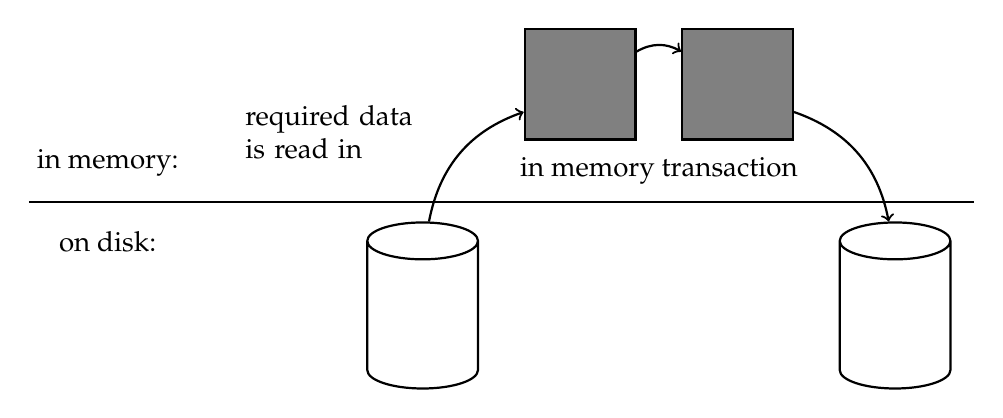
\begin{tikzpicture}
\begin{scope}[thick]

  % initial disk store
  \node[cylinder, aspect=2, rotate=90, draw, minimum height=60pt, minimum width=40pt] (disk1)
        at (2,0) {};
  \node[right] at (disk1.south east) {};

  % dividing line
  \draw (-3,1.5) -- (9,1.5);
  \draw (-2.0,2.0) node {in memory:};
  \draw (-2.0,1.0) node {on disk:};


  \begin{scope}[yshift=3cm, xshift=4cm]
  \node[rectangle, draw, minimum width=40pt, minimum height=40pt, fill=gray]
       (state1) at (0,0) {};
  \end{scope}

  \path[->] (disk1) edge[bend left] node[above left=-0.3cm, text width=80pt]
                    {required data \\ is read in} (state1);

  \begin{scope}[yshift=3cm, xshift=6cm]
  \node[rectangle, draw, minimum width=40pt, minimum height=40pt, fill=gray]
       (state2) at (0,0) {};
  \end{scope}

  \path[->] (state1) edge[bend left] node[below=1.3cm] {in memory transaction} (state2);

  % final disk store
  \node[cylinder, aspect=2, rotate=90, draw, minimum height=60pt, minimum width=40pt] (disk2)
        at (8,0) {};

  \path[->] (state2) edge[bend left] (disk2);

\end{scope}
\end{tikzpicture}
\end{center}

As an example of this, consider validating a ledger transaction including its
UTxO inputs: we know we will need to look up the transaction inputs in the UTxO
mapping. Which inputs we will need is clearly known in advance as they are
explicit in the transaction itself. For the Cardano ledger rules in general, we
believe that we can determine all the required mapping entries and that there
are no dynamic dependencies that cannot be discovered in advance. This fact will
enable us to keep the design simpler.

We do not use a cache (or anti-cache): we will \emph{always} read the required
data into memory. As we have discussed previously \citep{utxo-db} the data
access patterns do not substantially benefit from caching. This choice keeps
the design simpler.

\subsection{Differences of data structures}
\label{differences-of-data-structures}

We will make use of \emph{differences} of data structures. In particular,
we will arrange for the ledger rules to return differences and it is these
differences that can be applied to the on-disk data structures (e.g. as inserts,
updates and deletes for on-disk tables).

\begin{center}
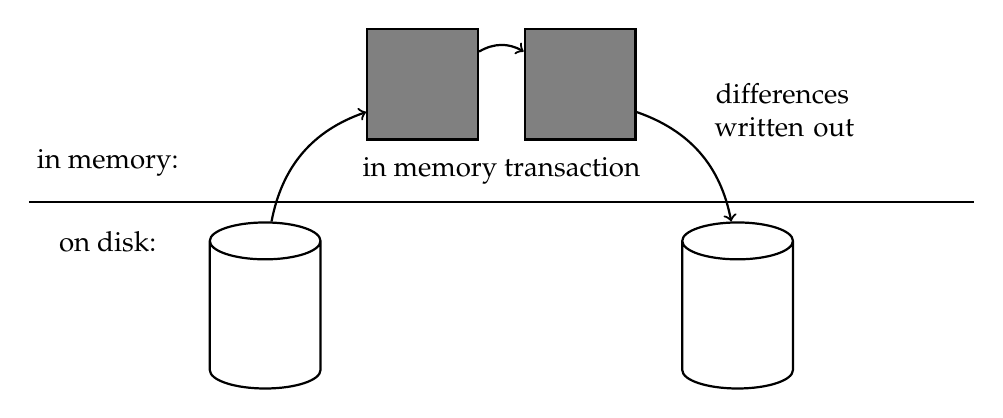
\begin{tikzpicture}
\begin{scope}[thick]

  % initial disk store
  \node[cylinder, aspect=2, rotate=90, draw, minimum height=60pt, minimum width=40pt] (disk1)
        at (0,0) {};
  \node[right] at (disk1.south east) {};

  % dividing line
  \draw (-3,1.5) -- (9,1.5);
  \draw (-2.0,2.0) node {in memory:};
  \draw (-2.0,1.0) node {on disk:};


  \begin{scope}[yshift=3cm, xshift=2cm]
  \node[rectangle, draw, minimum width=40pt, minimum height=40pt, fill=gray]
       (state1) at (0,0) {};
  \end{scope}

  \path[->] (disk1) edge[bend left] (state1);

  \begin{scope}[yshift=3cm, xshift=4cm]
  \node[rectangle, draw, minimum width=40pt, minimum height=40pt, fill=gray]
       (state2) at (0,0) {};
  \end{scope}

  \path[->] (state1) edge[bend left] node[below=1.3cm] {in memory transaction} (state2);

  % final disk store
  \node[cylinder, aspect=2, rotate=90, draw, minimum height=60pt, minimum width=40pt] (disk2)
        at (6,0) {};

  \path[->] (state2) edge[bend left] node[above right=0.1cm, text width=80pt] {differences \\ written out} (disk2);

\end{scope}
\end{tikzpicture}
\end{center}

The simplest scheme, as in the diagram above, would be to write differences
back to disk immediately. As we will discuss, we will actually want to hold
the differences in memory across many transactions and flush them to disk later.

\subsection{Partitioned in-memory/on-disk representation}
\label{partitioned-representation}

To meet our targets for memory use, we must keep the bulk of the ledger state on
disk, but as mentioned already in \cref{anti-caching}, it is not necessary to
keep the \emph{entire} ledger state on disk. We can achieve a substantially
simpler design if we partition the state such that \emph{only} large key-value
mappings are kept on disk, and all other data remains in memory. This approach
is simpler in several ways.
\begin{itemize}
\item Rather than solve the general problem of keeping complex compound data on
      disk, we can reduce it to the well-understood problem of on-disk
      key-value stores.
\item As mentioned in \cref{reading-data-into-memory-in-advance}, we need to be
      able to predict which parts of the ledger state will need to be fetched
      from disk. If it is only the large mappings that are on disk, then we do
      not need to consider which other `miscellaneous' parts of the ledger
      state are needed since those parts are always in memory. This
      substantially simplifies the problem.
\item As mentioned in \cref{differences-of-data-structures}, we need to be able
      to represent and manage differences of data kept on disk. Differences of
      key-value mappings are straightforward, so we can avoid the general
      problem of differences of complex data structures.
\end{itemize}

The observation that we have made about the Cardano ledger state is that while
its structure is relatively complex, with many nested parts, most of it is
relatively small. Only a few parts of the ledger state are really large, and
those parts are all finite mappings. Thus, we believe this approach will be
sufficient to ensure the memory needed remains within the memory available. The
requirements for scale and resource use are given in the previous document
\citep[Section 3]{utxo-db}.

Furthermore, all the large finite mappings in the ledger state have relatively
simple key and value types that can be represented as short byte strings. This
allows them to be represented as on-disk key-value stores, which gives us a
wide choice of store implementations. Previous analysis \citep[Section 5]{utxo-db}
indicates that the performance requirements of the different mappings are all
compatible, so we believe we can use a single key-value store implementation
for all the on-disk mappings.

As for what counts as a large mapping, we draw the dividing line between `large'
and `small' between those that are proportional to the number of stake addresses
(or bigger) and those that are proportional to the number of stake pools (or
smaller). That is, mappings with sizes proportional to the number of stake pools
-- or something smaller than the number of stake pools -- will be kept in
memory. On the other hand mappings with sizes proportional to the number of
stake address -- or bigger than the number of stake addresses -- should be kept
on disk. The table below lists a selection of important mappings, what their
size is proportional to, and whether they will be stored in memory or
(primarily) on disk.
\begin{center}
\begin{tabular}{lll}
Mapping: & Size proportional to: & Location: \\
\hline \hline \\
The UTxO                              & number of UTxO entries    & on disk \\
Delegation choices                    & number of stake addresses & on disk \\
Reward account balances               & number of stake addresses & on disk \\
Stake address pointers                & number of stake addresses & on disk \\
Stake distribution (by stake address) & number of stake addresses & on disk \\
\hline \\
Stake distribution (by pool)          & number of stake pools & in memory \\
Stake pool parameters                 & number of stake pools & in memory \\
Protocol parameters                   & constant              & in memory
\end{tabular}
\end{center}
In particular, note that the consensus layer needs rapid and random access to
the stake distribution (by block producer, i.e, stake pool) to be able to
validate block headers. Therefore, performance concerns dictate that at least
one mapping proportional to the number of stake pools needs to be kept in
memory.

For mappings based on the same key, it may or may not make sense to combine them
into a single on-disk store. Combining them may save space but depending on the
access pattern and on-disk store implementation we may obtain better
performance by keeping them separate.

In a design where the state is partitioned between large on-disk tables and all
other state in memory, the pattern for performing a transaction is as depicted
below. We read the required data from the on-disk tables and combine it with the
in-memory state to give a combined state that we can use to perform the
transaction. The transaction result is split again between the new in-memory
state, and differences on the large mappings which can be applied to the
on-disk tables.

\begin{center}
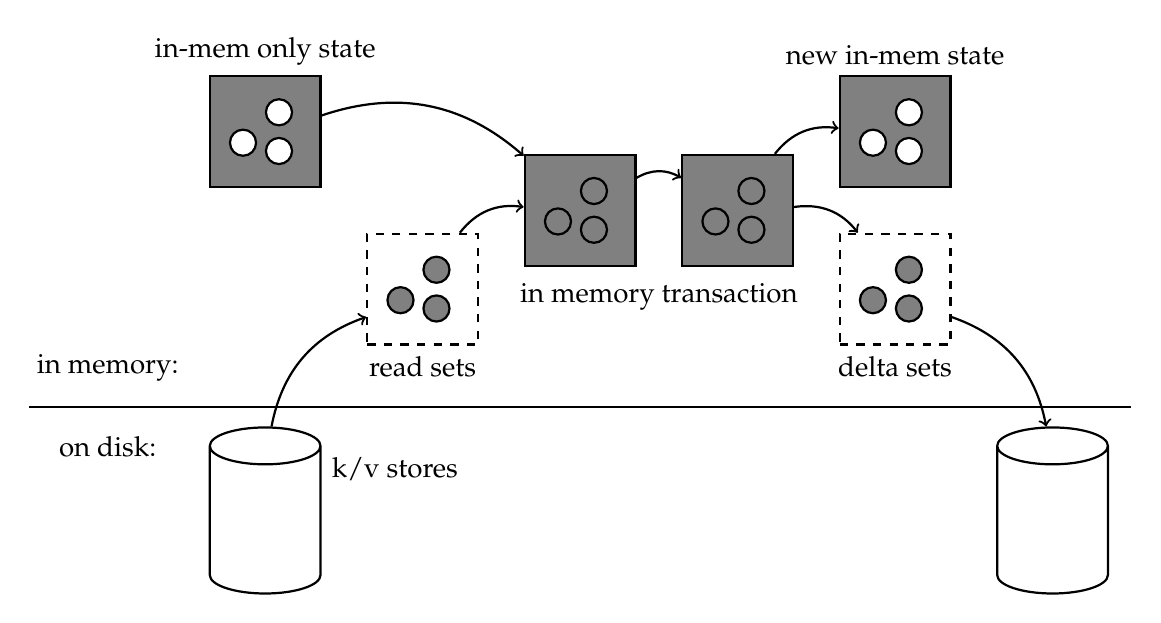
\begin{tikzpicture}
\begin{scope}[thick]

  % initial disk store
  \node[cylinder, aspect=2, rotate=90, draw, minimum height=60pt, minimum width=40pt] (disk1)
        at (0,0) {};
  \node[right] at (disk1.south east) {k/v stores};

  % dividing line
  \draw (-3,1.5) -- (11,1.5);
  \draw (-2.0,2.0) node {in memory:};
  \draw (-2.0,1.0) node {on disk:};

  \begin{scope}[yshift=5cm]
  \node[rectangle, draw, minimum width=40pt, minimum height=40pt, fill=gray]
       (inmem1) at (0,0) {};
  \node[above] at (inmem1.north) {in-mem only state};
  \node[circle, draw, minimum width=5pt, fill=white] at (-8pt,-4pt) {};
  \node[circle, draw, minimum width=5pt, fill=white] at ( 5pt, 7pt) {};
  \node[circle, draw, minimum width=5pt, fill=white] at ( 5pt,-7pt) {};
  \end{scope}

  \begin{scope}[yshift=3cm, xshift=2cm]
  \node[rectangle, draw, dashed, minimum width=40pt, minimum height=40pt]
       (readset) at (0,0) {};
  \node[below] at (readset.south) {read sets};
  \node[circle, draw, minimum width=5pt, fill=gray] at (-8pt,-4pt) {};
  \node[circle, draw, minimum width=5pt, fill=gray] at ( 5pt, 7pt) {};
  \node[circle, draw, minimum width=5pt, fill=gray] at ( 5pt,-7pt) {};
  \end{scope}

  \path[->] (disk1) edge[bend left] (readset);

  \begin{scope}[yshift=4cm, xshift=4cm]
  \node[rectangle, draw, minimum width=40pt, minimum height=40pt, fill=gray]
       (state1) at (0,0) {};
  \node[circle, draw, minimum width=5pt] at (-8pt,-4pt) {};
  \node[circle, draw, minimum width=5pt] at ( 5pt, 7pt) {};
  \node[circle, draw, minimum width=5pt] at ( 5pt,-7pt) {};
  \end{scope}

  \path[->] (inmem1) edge[bend left] (state1);
  \path[->] (readset) edge[bend left] (state1);

  \begin{scope}[yshift=4cm, xshift=6cm]
  \node[rectangle, draw, minimum width=40pt, minimum height=40pt, fill=gray]
       (state2) at (0,0) {};
  \node[circle, draw, minimum width=5pt] at (-8pt,-4pt) {};
  \node[circle, draw, minimum width=5pt] at ( 5pt, 7pt) {};
  \node[circle, draw, minimum width=5pt] at ( 5pt,-7pt) {};
  \end{scope}

  \path[->] (state1) edge[bend left] node[below=1.3cm] {in memory transaction} (state2);

  \begin{scope}[yshift=5cm, xshift=8cm]
  \node[rectangle, draw, minimum width=40pt, minimum height=40pt, fill=gray]
       (inmem2) at (0,0) {};
  \node[above] at (inmem2.north) {new in-mem state};
  \node[circle, draw, minimum width=5pt, fill=white] at (-8pt,-4pt) {};
  \node[circle, draw, minimum width=5pt, fill=white] at ( 5pt, 7pt) {};
  \node[circle, draw, minimum width=5pt, fill=white] at ( 5pt,-7pt) {};
  \end{scope}

  \begin{scope}[yshift=3cm, xshift=8cm]
  \node[rectangle, draw, dashed, minimum width=40pt, minimum height=40pt]
       (deltaset) at (0,0) {};
  \node[below] at (deltaset.south) {delta sets};
  \node[circle, draw, minimum width=5pt, fill=gray] at (-8pt,-4pt) {};
  \node[circle, draw, minimum width=5pt, fill=gray] at ( 5pt, 7pt) {};
  \node[circle, draw, minimum width=5pt, fill=gray] at ( 5pt,-7pt) {};
  \end{scope}

  \path[->] (state2) edge[bend left] (inmem2);
  \path[->] (state2) edge[bend left] (deltaset);

  % final disk store
  \node[cylinder, aspect=2, rotate=90, draw, minimum height=60pt, minimum width=40pt] (disk2)
        at (10,0) {};

  \path[->] (deltaset) edge[bend left] (disk2);

\end{scope}
\end{tikzpicture}
\end{center}

Finally, note that for the parts of the ledger state that are kept in memory,
there does still need to be a mechanism to restore the state when the node
restarts. The intention is to use the same approach as the consensus layer uses
now: writing snapshots to disk from time to time and replaying from the most
recent snapshot upon start up. Only minor changes to this scheme are necessary
to account for the on-disk mappings. To achieve a consistent snapshot of the
overall state, it will be necessary to take snapshots of the on-disk mappings
and of the in-memory data for the exact same state (i.e., corresponding to the
ledger state of the same chain). If the snapshots of the on-disk and in-memory
parts were not synchronised, it would not be possible to replay the subsequent
changes upon start-up.

\subsection{Access to multiple (logical) ledger states}
\label{access-to-multiple-logical-ledger-states}

As discussed in \cref{ledger-state-handling-in-the-current-consensus-layer},
the consensus design relies on having efficient access to multiple ledger
states corresponding to the $k$ most recent blocks on the current chain.
Furthermore, the chain selection algorithm needs to compute ledger states along
candidate chains without yet committing to them. Evaluating the validity of
candidate chains involves computing the ledger state block by block, but if
the chain turns out to be invalid, then we must discard it and the corresponding
ledger state. In particular, in this situation we must not change our current
chain or its corresponding ledger state.

Thus, the consensus design demands that we have the ability to manipulate
multiple logical ledger states. On the face of it, this requirement would appear
to be hard to satisfy using traditional on-disk data structures or database
management systems which only provide a single `current' value.

We also discussed in \cref{ledger-state-handling-in-the-current-consensus-layer}
that the existing consensus design relies on persistent data structures so that
keeping many ledger states costs little more than keeping a single state. We noted that
the incremental cost of each extra copy is proportional to the differences
between the states. Of course, this only works because the states are
\emph{closely related}. More specifically, all the ledger states the node needs
to keep around are derived from a common state: the ledger state of the `immutable
tip' of the current chain. This is the ledger state for the tip of the chain if
were to remove the most recent $k$ blocks. Obviously, all the ledger states for
the last $k$ blocks are related to this state by application of the ledger
rules. The same holds for the ledger states of any candidate chains that we
need to validate since they must have an intersection within the last $k$
blocks.

\begin{center}
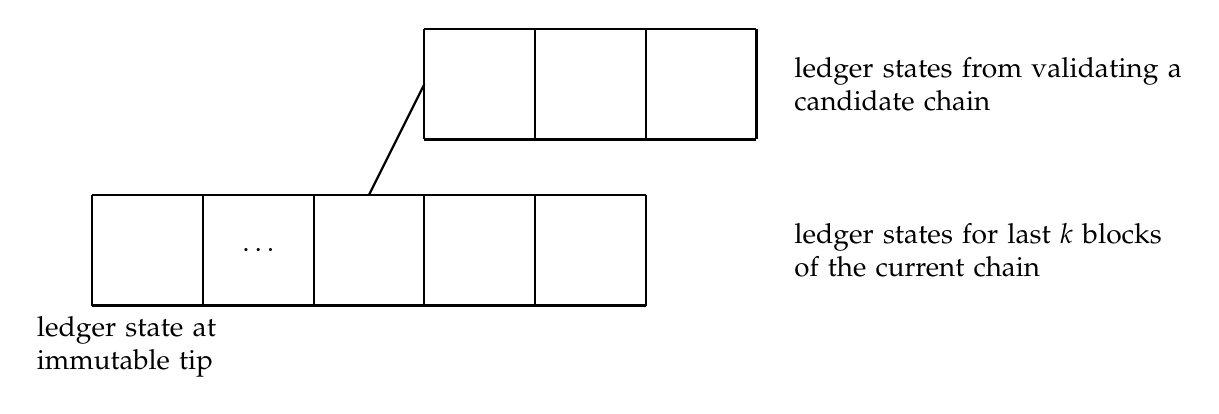
\begin{tikzpicture}
\begin{scope}[thick]

\draw[step=40pt] (0,0) grid (200pt,40pt);
\node[text width=80pt, anchor=north] at (20pt, 0pt)
     {ledger state at immutable tip};
\node at (60pt, 20pt) {$\ldots$};
\node[text width=140pt, anchor=west] at (250pt, 20pt)
     {ledger states for last $k$ blocks of the current chain};

\draw[step=40pt, yshift=60pt] (120pt, 0pt) grid (240pt,40pt);
\draw (120pt, 80pt) -- (100pt, 40pt);
\node[text width=140pt, anchor=west] at (250pt, 80pt)
     {ledger states from validating a candidate chain};

\end{scope}
\end{tikzpicture}
\end{center}
In summary, we know that the differences between all the ledger states that we
need to manipulate are relatively small (compared to the size of the ledger
state itself), and they are all derived from one ledger state at the `immutable
tip'. Using persistent data structures is one way to take advantage of this
property. Another way is to \emph{represent the differences explicitly} and
use that to construct (on-demand) the multiple logical states (or parts
thereof).

The design we choose to take is as follows:
\begin{itemize}
\item we will keep a single copy of the ledger state (k/v mappings) on disk;
\item that copy will correspond to the ledger state at the immutable tip, which
      is the common root point of all other states;
\item we will represent all other derived ledger states using differences from
      the common state;
\item all these differences will be maintained in memory.
\end{itemize}
Or in diagram form:
\begin{center}
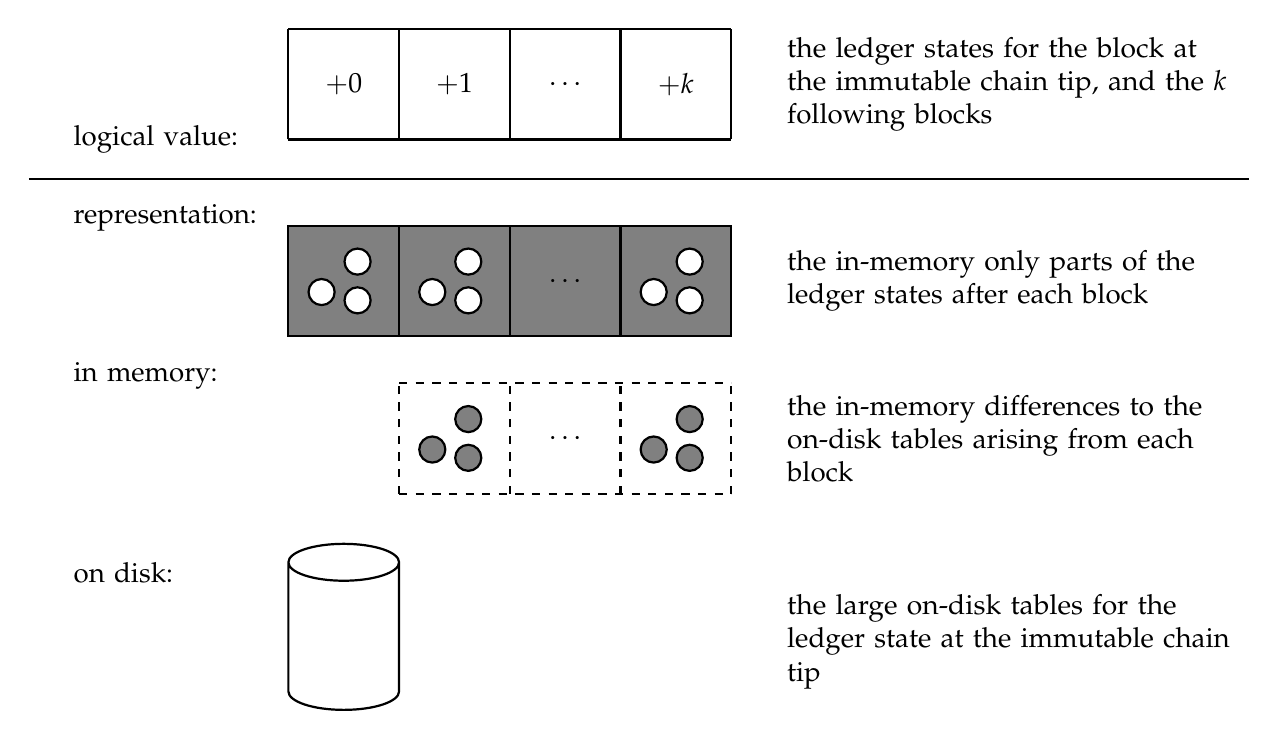
\begin{tikzpicture}
\begin{scope}[thick]

  % disk icon
  \node[cylinder, aspect=2, rotate=90, draw, minimum height=60pt, minimum width=40pt]
       (disk) at (0,-25pt) {};
  \draw (5.5cm, -25pt) node[align=left, anchor=west, text width=160pt]
        {the large on-disk tables for the ledger state at the immutable chain tip};

  \begin{scope}[yshift=3cm, xshift=0pt]
  \draw[step=40pt,xshift=-20pt, fill=gray] (0,0) grid (160pt,40pt) rectangle (0,0);
  \begin{scope}[xshift=0pt, yshift=20pt]
    \node[circle, draw, fill=white] at (-8pt,-4pt) {};
    \node[circle, draw, fill=white] at ( 5pt, 7pt) {};
    \node[circle, draw, fill=white] at ( 5pt,-7pt) {};
  \end{scope}
  \begin{scope}[xshift=40pt, yshift=20pt]
    \node[circle, draw, fill=white] at (-8pt,-4pt) {};
    \node[circle, draw, fill=white] at ( 5pt, 7pt) {};
    \node[circle, draw, fill=white] at ( 5pt,-7pt) {};
  \end{scope}
  \draw (80pt,  20pt) node {$\ldots$};
  \begin{scope}[xshift=120pt, yshift=20pt]
    \node[circle, draw, fill=white] at (-8pt,-4pt) {};
    \node[circle, draw, fill=white] at ( 5pt, 7pt) {};
    \node[circle, draw, fill=white] at ( 5pt,-7pt) {};
  \end{scope}
  \end{scope}
  \draw (5.5cm, 3cm+20pt) node[align=left, anchor=west, text width=160pt]
        {the in-memory only parts of the ledger states after each block};

  \begin{scope}[yshift=1cm, xshift=40pt]
  \draw[step=40pt,xshift=-20pt, dashed] (0,0) grid (120pt,40pt);
  \begin{scope}[xshift=0pt, yshift=20pt]
    \node[circle, draw, fill=gray] at (-8pt,-4pt) {};
    \node[circle, draw, fill=gray] at ( 5pt, 7pt) {};
    \node[circle, draw, fill=gray] at ( 5pt,-7pt) {};
  \end{scope}
  \draw (40pt,  20pt) node {$\ldots$};
  \begin{scope}[xshift=80pt, yshift=20pt]
    \node[circle, draw, fill=gray] at (-8pt,-4pt) {};
    \node[circle, draw, fill=gray] at ( 5pt, 7pt) {};
    \node[circle, draw, fill=gray] at ( 5pt,-7pt) {};
  \end{scope}
  \end{scope}
  \draw (5.5cm, 1cm+20pt) node[align=left, anchor=west, text width=160pt]
        {the in-memory differences to the on-disk tables arising from each block};

  % dividing line and text
  \begin{scope}[text width=70pt, align=left]
  \draw (-4,5) -- (11.5,5);
  \draw (-2.2,5.5) node {logical value:};
  \draw (-2.2,4.5) node {representation:};
  \draw (-2.2,2.5) node {in memory:};
  \draw (-2.2,0)   node {on disk:};
  \end{scope}

  % logical value
  \begin{scope}[yshift=5.5cm]
  \draw[step=40pt,xshift=-20pt] (0,0) grid (160pt,40pt);

  \draw[step=40pt,xshift=-20pt] (0,0) grid (160pt,40pt);
  \draw (0,     20pt) node {$+0$};
  \draw (40pt,  20pt) node {$+1$};
  \draw (80pt,  20pt) node {$\ldots$};
  \draw (120pt, 20pt) node {$+k$};

  \end{scope}
  \draw (5.5cm, 5.5cm+20pt) node[align=left, anchor=west, text width=160pt]
        {the ledger states for the block at the immutable chain tip,
         and the $k$ following blocks};

\end{scope}
\end{tikzpicture}
\end{center}

This design resolves the tension: it uses only a single on-disk value at any one
time, which lets us use traditional database techniques, and yet it also lets
us efficiently work with multiple logical values of the database state at once.

We must, of course, assess the memory use of this approach. It involves keeping
the changes from the last $k$ blocks in memory. Rough estimates suggest that, by
the time we hit the stretch target of 200 TPS, we should expect the
representation of the differences to require in the order of a few gigabytes of
memory. As we noted previously \citep[section 3.3.5]{utxo-db}, it would be
impractical to operate a public system at such TPS rates because of the high
resource use, but private instances may be practical and in such cases using a
few GB of memory would be acceptable.


\subsection{Enabling I/O pipelining}
\label{enabling-pipelining}

As discussed in the initial report \citep[sections 6.1 and 8.8]{utxo-db}, it is
expected that ultimately it will be necessary to make use of parallel I/O to
hit the stretch performance targets. This is because the expectation is that
disk I/O (rather than network or CPU) could well be the bottleneck for very
high throughput validation of blockchains.

We may not make use of parallelism in an initial implementation, but if we are
to keep open the option to use parallelism later, then it is necessary for the
interface between the application and the disk storage layer to expose the
opportunities for parallelism. Thus, we wish to find an interface that allows
for I/O parallelism.

It is worth keeping in mind how much parallel I/O we need to saturate a modern
SSD. It is in the order of 32 -- 64 concurrent I/O operations being performed
at all times. A useful abstraction is to think of it as a queue of in-progress
operations where new I/O operations are added at one end and results arrive
eventually at the other end, and the queue should be kept sufficiently full to
saturate the SSD's throughput. Due to the high throughput and timing jitter, it
is better to `over-fill' the queue by some amount, e.g., $2\times$. That is, in
order to ensure the SSD queue `depth' does not drain to below 64, it may be necessary to aim to keep double that number of
operations in progress at the application level. The appropriate amount to use can be tuned based on I/O
profiling tools, but the overall point is clear: to fully exploit the
throughput of an SSD, we need to keep a substantial number of operations in
progress at once -- and on a continuous basis.

Since blockchains are mostly linear in nature (being a chain), the opportunities
for I/O parallelism come from batching and pipelining.
\begin{description}
\item[Batching:] This is submitting a batch of I/O operations and waiting to
                collect them all. For example, we could submit all the I/O
                reads for a single block in one go.

                A block with 64 transactions with 2 UTxO inputs each would
                generate 128 read I/O operations. So, we can see that large enough blocks
                could individually temporarily saturate an SSD. Note that with
                just batching there is no overlapping of computation with I/O
                since we wait for the I/O to complete and then use the results.

\item[Pipelining:] This is submitting a (typically) continuous stream of I/O
                operations in advance of when their results are needed, and
                collecting each result (usually) in time before it is needed.

                For example, while we are doing the CPU work to process one
                block, we can have submitted the I/O operations for one or more
                subsequent blocks so that their results are available by the
                time we come to process them.

                Note that this involves overlapping computation with I/O.
                In principle, the I/O queue can be kept full: we can avoid
                any gaps between blocks when no I/O is being performed.
\end{description}
Given this, it is clear that pipelining is superior in terms of achieving
enough I/O parallelism to saturate an SSD, but is also clear that it is more
complex to arrange. The opportunity for batching arises naturally from
processing blocks as a unit. In practice, if pipelining is used, it would also
be used with batching as a pipeline of batches (per block).

For this stage of the design, we simply need to ensure that the
scheme for disk I/O makes it possible to take advantage of I/O pipelining.
Where it is practical to take advantage of pipelining is then a design decision
for the consensus layer. It may only be worth attempting to use pipelining for
bulk sync situations, and not attempting to use it opportunistically such as
when switching forks. Using only batching is likely to be sufficient for normal
operation when the node is already in sync. Indeed, using only batching may be
sufficient for an initial integration that is not yet aiming for the higher
throughput targets.

\section{Notation and properties of differences}
\label{notation-differences}

To make the design ideas from the previous section more precise, we will use a
more formal presentation of differences.
In this section, we briefly review the notation and properties of differences
that we will use in later sections. We roughly follow the presentation by
\citet{change-calculus}.

We start with a set $A$ of values of our data structure of interest. For some
sets\footnote{Our data structures of interest will typically be
finite mappings, and we will see that differences for
finite mappings are straightforward.}, we are able to find a corresponding
set $\Delta{A}$ of \emph{differences} or \emph{changes} on values from the set
$A$. We will use a naming convention $\deltavar{a} \in \Delta{A}$, using a
$\Delta$-accent, to remind ourselves which variables represent differences.
So note that $\deltavar{a}$ is not an operator on a variable $a$, as it is simply a
variable naming convention.

We can \emph{apply} a difference to a value to produce a new value: given
$a \in A$ and $\deltavar{a} \in \Delta{A}$, we can use the apply operator
$\triangleleft$ to give us $(a \triangleleft \deltavar{a}) \in A$.

The differences $\Delta{A}$ form a monoid with an associative operator
$\diamond$ and a zero element $\mathbf{0} \in \Delta{A}$. This means we can
compose changes, and we can always have no change.

In addition to the monoid laws, we have a couple of straightforward laws involving
applying changes. The zero change is indeed no change at all
\begin{equation}
  \forall a \in A. ~~ a \triangleleft \mathbf{0} = a
\end{equation}
and applying multiple changes is the same as applying the composition of the
changes.
\begin{equation}
\label{eq:apply-compose}
  \forall a \in A. ~~ \forall \deltavar{b}, \deltavar{c} \in \Delta{A}. ~~
    (a \triangleleft \deltavar{b}) \triangleleft \deltavar{c}
  = a \triangleleft (\deltavar{b} \diamond \deltavar{c})
\end{equation}
We will use the notation $\Diamond\hspace{-3pt}\sum$ for an n-way monoidal sum,
meaning simply the repeated use of the associative $\diamond$ operator. An empty
0-way sum is of course defined as the zero change.
\[
\Diamond\hspace{-4pt}\sum_{i=0}^n{\deltavar{a}_i}
= \deltavar{a}_0 \diamond \deltavar{a}_1 \diamond \deltavar{a}_2 \diamond \ldots \deltavar{a}_n
\]
We will also talk about functions that transform values, and corresponding
functions that compute differences. Given a function $f : A \to A$, a
difference function $\deltavar{f} : A \to \Delta{A}$ corresponds to the
original function $f$ if it satisfies the property that applying the change
gives the same result as the original function.
\begin{equation}
  a \triangleleft \deltavar{f}(a) = f(a)
\end{equation}
We will sometimes be able to derive difference functions from the original
transformation functions.


\section{Abstract models of hybrid on-disk/in-memory databases}
\label{abstract-models}

In this section, we will look at an abstract formal treatment of databases based
on differences. The abstract models we will look at are motivated by the ideas
discussed in \cref{general-approach}. We will discuss how different models
correspond to different implementation strategies, including in-memory and
on-disk data storage. Where appropriate and possible, we will sketch proofs to
reassure ourselves that we will get correct results. There are a few reasons to
consider these models.
\begin{description}
\item[Lucid descriptions]
There is the usual reason for abstraction, that omitting unnecessary details can
make the ideas easier and shorter to describe.

\item[Imagining implementation strategies]
Another reason is that, although these are abstract models, they can be seen
to correspond to certain implementation approaches. For example, we will refer
to certain terms as representing on-disk or in-memory data structures. Obviously,
mathematically there is no such distinction, but it is very useful to see the
correspondence to an implementation strategy. It lets us think about
implementation constraints and whether a design idea seems plausible.

\item[Seeing equivalences]
By describing the models in mathematical terms, we may be able to show
mathematical equivalences between models. This is especially useful when we
have a model that corresponds to a preferred implementation approach and we
can show that it is mathematically equivalent to some reference model.
\end{description}
As mentioned in \cref{terminology}, our use of the term `database' in this
section is quite abstract: we mean only some collection of data. This section
makes use of the idea and notation of the calculus of differences from the
previous section.

\subsection{Simple sequential databases}
\label{simple-sequential-databases}

This is a very simple model. In this model, there is an initial database state
$\mathit{db}_0 \in \mathit{DB}$ and a series of state transformation functions
$\mathit{tx}_0, \mathit{tx}_1, \ldots \in \mathit{DB} \to \mathit{DB}$, which we can also think of as database
transactions. Applying each transformation function to the previous state by
$\mathit{db}_{n+1} = \mathit{tx}_n(\mathit{db}_n)$ gives rise to a series of database states
$\mathit{db}_0, \mathit{db}_1, \ldots$.

\begin{center}
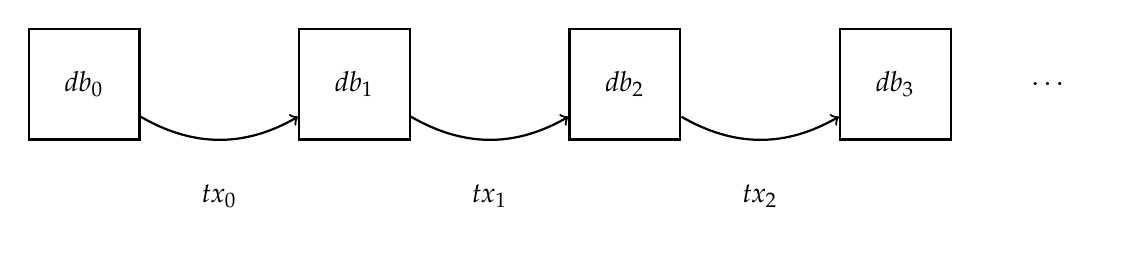
\begin{tikzpicture}[state/.style={rectangle, draw}]
\begin{scope}[thick, minimum width=40pt, minimum height=40pt]
  \node[state]   (db0)                      {$\mathit{db}_0$};
  \node[state]   (db1) [right=2.0cm of db0] {$\mathit{db}_1$};
  \node[state]   (db2) [right=2.0cm of db1] {$\mathit{db}_2$};
  \node[state]   (db3) [right=2.0cm of db2] {$\mathit{db}_3$};
  \node                [right=0.5cm of db3] {$\ldots$};

  \path[->] (db0) edge [bend right] node[below] {$\mathit{tx}_0$} (db1);
  \path[->] (db1) edge [bend right] node[below] {$\mathit{tx}_1$} (db2);
  \path[->] (db2) edge [bend right] node[below] {$\mathit{tx}_2$} (db3);
\end{scope}
\end{tikzpicture}
\begin{align*}
  \mathit{db}_1 & = \mathit{tx}_0(\mathit{db}_0) \\
  \mathit{db}_2 & = \mathit{tx}_1(\mathit{db}_1) \\
  \vdots
\end{align*}
And in general
\begin{equation}
\label{eq:sequential-recurrence}
\mathit{db}_{i+1} = \mathit{tx}_i(\mathit{db}_i)
\end{equation}
\end{center}
This model serves as an important semantic reference point for the more
complicated models below. We will want to show that some of our more
complicated models are semantically equivalent to this simple one.

If we think of this model in terms of what kind of implementation strategy it
most clearly represents, then it would be a simple in-memory design. That is a
design where the whole database is a simple program value that is transformed
with pure functions.

\subsection{Change-based databases}
\label{change-based-databases}

In this model, we want to introduce two concepts:
\begin{enumerate}
\item the use of transaction difference functions and applying differences; and
\item identifying the subset of values that each transaction needs.
\end{enumerate}
It is otherwise just a simple sequence of database values. The use of these two
concepts makes this a simple but reasonable model of an on-disk database with
in-memory transaction processing (as introduced in
\cref{reading-data-into-memory-in-advance,differences-of-data-structures}).
Using a subset of values corresponds to reading the data in from disk, while
obtaining and applying differences corresponds to writing changes back to disk.

Whereas in the previous model we had a series of transaction functions
$\mathit{tx}_0, \mathit{tx}_1, \ldots$, in this model we will have difference
functions
$\deltavar{\mathit{tx}}_0, \deltavar{\mathit{tx}}_1, \ldots : \mathit{DB} \to \Delta\mathit{DB}$. These are required to be proper difference functions, satisfying the property
\begin{equation}
\label{eq:diff-fun}
db \triangleleft \deltavar{\mathit{tx}}(\mathit{db}) = \mathit{tx}(\mathit{db})
\end{equation}

For each transaction, we will also identify the subset of the database state that
the transaction needs. This will typically take the form of a set of keys
$\mathit{ks} \subseteq \dom{\mathit{DB}}$ (or collection of sets of keys) which will be used to
perform a domain restriction $\restrict{\mathit{db}}{\mathit{ks}} \subseteq \mathit{DB}$.
So, there will key sets $\mathit{ks}_0, \mathit{ks}_1, \ldots$ corresponding to
the transactions $\deltavar{\mathit{tx}}_0, \deltavar{\mathit{tx}}_1, \ldots$.
We will require that the transaction really does only make use of the subset
by requiring the property that the transaction function gives the same result
on the subset as on the whole state
\begin{equation}
\label{eq:tx-within-keyset}
  \deltavar{\mathit{tx}}(\restrict{\mathit{db}}{\mathit{ks}}) = \deltavar{\mathit{tx}}(\mathit{db})
\end{equation}
The domain restriction on the database value corresponds to reading a set of
keys $\mathit{ks}$ from the database, and we call the result a \emph{read set}.
We will define each read set as
$\mathit{rs}_i = \restrict{\mathit{db}_i}{\mathit{ks}_i}$
and the changes from each transaction as
$\deltavar{\mathit{db}}_{i+1} = \deltavar{\mathit{tx}}_i(\mathit{rs}_i)$.
The series of database states
$\mathit{db}_0, \mathit{db}_1, \ldots$ can now be constructed by applying the changes from each
transaction to the previous database state.
\begin{center}
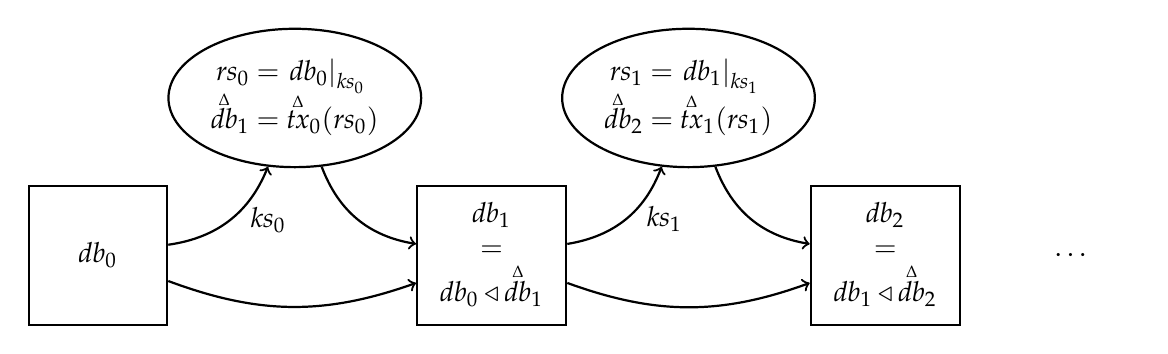
\begin{tikzpicture}
\begin{scope}[thick, rectangle, minimum width=50pt, minimum height=50pt]
  \node[draw] (db0)           {$\mathit{db}_0$};
  \node[draw] (db1) at (5,0)  {$\eqabove{\mathit{db}_1}{\mathit{db}_0 \triangleleft \deltavar{\mathit{db}}_1}$};
  \node[draw] (db2) at (10,0) {$\eqabove{\mathit{db}_2}{\mathit{db}_1 \triangleleft \deltavar{\mathit{db}}_2}$};
  \node[right=0.5cm of db2] {$\ldots$};

  % read sets and transaction differences
  \node[ellipse, draw, inner sep=-3pt] (rs0) at (2.5cm, 2cm)
       {$\begin{array}{r@{~=~}l}
           \mathit{rs}_0 & \restrict{\mathit{db}_0}{\mathit{ks}_0} \\
           \deltavar{\mathit{db}}_1 & \deltavar{\mathit{tx}}_0(\mathit{rs}_0)
         \end{array}$};
  \node[ellipse, draw, inner sep=-3pt] (rs1) at (7.5cm, 2cm)
       {$\begin{array}{r@{~=~}l}
           \mathit{rs}_1 & \restrict{\mathit{db}_1}{\mathit{ks}_1} \\
           \deltavar{\mathit{db}}_2 & \deltavar{\mathit{tx}}_1(\mathit{rs}_1)
         \end{array}$};

  \path[->] (db0) edge [bend right] node[right=-0.4] {$\mathit{ks}_0$} (rs0);
  \path[->] (db1) edge [bend right] node[right=-0.4] {$\mathit{ks}_1$} (rs1);

  \path[->] (rs0) edge [bend right] (db1);
  \path[->] (rs1) edge [bend right] (db2);

  \path[->] (db0) edge [bend right=20] (db1);
  \path[->] (db1) edge [bend right=20] (db2);
\end{scope}
\end{tikzpicture}
\begin{equation*}
\begin{array}{c@{~}l@{\quad}l@{\quad}l}
  \mathit{db}_1 & = \mathit{db}_0 \triangleleft \deltavar{\mathit{db}}_1
                & \mathbf{where} \quad \deltavar{\mathit{db}}_1 = \deltavar{\mathit{tx}}_0(\mathit{rs}_0)
                & \mathbf{and} \quad \mathit{rs}_0 = \restrict{\mathit{db}_0}{\mathit{ks}_0} \\
  \mathit{db}_2 & = \mathit{db}_1 \triangleleft \deltavar{\mathit{db}}_2
                & \mathbf{where} \quad \deltavar{\mathit{db}}_2 = \deltavar{\mathit{tx}}_1(\mathit{rs}_1)
                & \mathbf{and} \quad \mathit{rs}_1 = \restrict{\mathit{db}_1}{\mathit{ks}_1} \\
\end{array}
\end{equation*}
\vdots \\
And in general
\begin{equation*}
\begin{array}{c@{~}l@{\quad}l@{\quad}l}
  \mathit{db}_{i+1} & = \mathit{db}_i \triangleleft \deltavar{\mathit{db}}_{i+1}
                    & \mathbf{where} \quad \deltavar{\mathit{db}}_{i+1} = \deltavar{\mathit{tx}}_i(\mathit{rs}_i)
                    & \mathbf{and} \quad \mathit{rs}_i = \restrict{\mathit{db}_i}{\mathit{ks}_i} \\
\end{array}
\end{equation*}
\end{center}

It is straightforward to see how this is equivalent to the simple model.

\begin{align*}
         & \mathit{db}_{i+1} = \mathit{db}_i \triangleleft \deltavar{\mathit{tx}}_i(\restrict{\mathit{db}_i}{\mathit{ks}_i}) \\
  \equiv & \quad \text{\{by the restriction property \cref{eq:tx-within-keyset} that
                      $\deltavar{\mathit{tx}}_i(\restrict{\mathit{db}}{\mathit{ks}_i}) = \deltavar{\mathit{tx}}_i(\mathit{db})$\}} \\
         & \mathit{db}_{i+1} = \mathit{db}_i \triangleleft \deltavar{\mathit{tx}}_i(\mathit{db}_i) \\
  \equiv & \quad \text{\{by the difference function property \cref{eq:diff-fun} that
                      $db \triangleleft \deltavar{\mathit{tx}}(\mathit{db}) = \mathit{tx}(\mathit{db})$\}} \\
         & \mathit{db}_{i+1} = \mathit{tx}_i(\mathit{db}_i)
\end{align*}

Which is the same as \cref{eq:sequential-recurrence}: the recurrence for the simple model.

\subsection{Hybrid on-disk / in-memory databases}
\label{sec:hybrid-on-disk-in-memory-db}

This model covers the bare essence of the idea from
\cref{access-to-multiple-logical-ledger-states}: that is, representing the
ledger state as the combination of data on disk and differences in memory. This
model is just about representing a \emph{single} ledger state. We will look at
representing \emph{multiple} states in \cref{multiple-logical-database-states}.

In this model, we represent the data as a combination of two parts. One will
stand for data on disk and the other will stand for data in memory. The on-disk part
will be ordinary database values
$\mathit{db}^{\mathrm{disk}}_i \in \mathit{DB}$, while the in-memory part will
be database differences
$\deltavar{\mathit{db}}^{\mathrm{mem}}_i \in \Delta{\mathit{DB}}$. We
define the  overall logical value of the database to be the on-disk part with
the in-memory changes applied `on top'.
\begin{equation}
\label{eq:hybrid-db}
\mathit{db}_i = \mathit{db}^{\mathrm{disk}}_i \triangleleft \deltavar{\mathit{db}}^{\mathrm{mem}}_i
\end{equation}
In a visual notation, we will depict that idea as follows. Above the line is
the logical value of the database, while below the line is the corresponding
representation.
\begin{center}
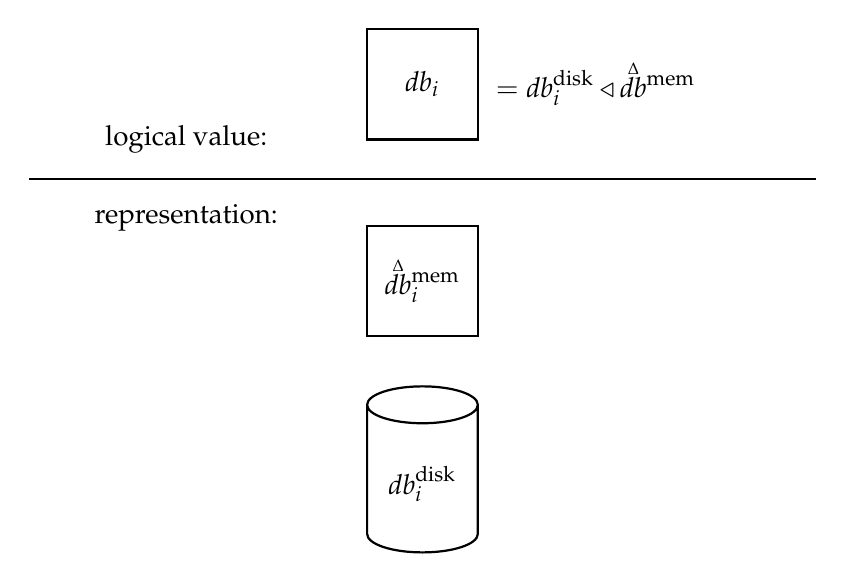
\begin{tikzpicture}
\begin{scope}[thick]

  % disk icon
  \node[cylinder, aspect=2, rotate=90, draw, minimum height=60pt, minimum width=40pt]
        at (0,-25pt) {};
  \draw (0, -25pt) node {$\mathit{db}^{\mathrm{disk}}_i$};

  % in memory
  \draw (-20pt,1) rectangle (20pt,1cm+40pt);
  \draw (0,1cm+20pt) node {$\deltavar{\mathit{db}}^{\mathrm{mem}}_i$};

  % dividing line
  \draw (-5,3) -- (5,3);
  \draw (-3,3.5) node {logical value:};
  \draw (-3,2.5) node {representation:};

  % logical value
  \draw (-20pt,3.5cm) rectangle (20pt,3.5cm+40pt);
  \draw (0,3.5cm+20pt) node {$\mathit{db}_i$};
  \draw (0.8,3.5cm+20pt) node[anchor=west] {$ = \mathit{db}^{\mathrm{disk}}_i \triangleleft \deltavar{\mathit{db}}^{\mathrm{mem}}$};
\end{scope}
\end{tikzpicture}
\end{center}

There are a couple of lemmas that will prove useful later when reasoning about
this representation. One is that if we have a domain restriction `outside' of
the application of changes, then it does not make any difference if we also use
domain restriction `inside' or not.
\begin{equation}
\label{eq:restriction}
  \restrict{\left(\mathit{db}_a \triangleleft \deltavar{\mathit{db}}_b\right)}{\mathit{ks}}
=
  \restrict{\left(\restrict{\mathit{db}_a}{\mathit{ks}} \triangleleft \deltavar{\mathit{db}}_b\right)}{\mathit{ks}}
\end{equation}
This lemma either needs to be proved universally or we will need to make it a
required property of the apply changes operator for the choice of $\Delta\mathit{DB}$.

The other useful lemma is a simple corollary of \cref{eq:tx-within-keyset} and
\cref{eq:restriction}
\begin{equation}
\label{eq:restriction_corollary}
  \deltavar{\mathit{tx}}\left(\restrict{\left(\mathit{db}_a \triangleleft \deltavar{\mathit{db}}_b\right)}{\mathit{ks}}\right)
=
  \deltavar{\mathit{tx}}\left(\restrict{\mathit{db}_a}{\mathit{ks}} \triangleleft \deltavar{\mathit{db}}_b\right)
\end{equation}
This lets us `shift' a domain restriction from outside to inside the application
of changes, within the context of a `proper' transaction function
$\deltavar{\mathit{tx}}$ that satisfies \cref{eq:tx-within-keyset}.

\subsubsection{Performing transactions}
\label{performing-transactions}
We now need to see how performing transactions works in this representation. We
will, of course, use the change-based style of transactions, as in the previous
model (in \cref{change-based-databases}). Given the changes
made by a transaction $\deltavar{\mathit{tx}}_i(\restrict{\mathit{db}_i}{\mathit{ks}_i})$,
we would normally obtain the new state of the database by applying the changes
to the previous state
\[
\mathit{db}_{i+1} = \mathit{db}_i \triangleleft \deltavar{\mathit{tx}}_i(\restrict{\mathit{db}_i}{\mathit{ks}_i})
\]
With the hybrid representation (for $\mathit{db}_i$), that is
\[
\mathit{db}_{i+1} = \left( \mathit{db}^{\mathrm{disk}}_i \triangleleft \deltavar{\mathit{db}}^{\mathrm{mem}}_i \right)
      \triangleleft \deltavar{\mathit{tx}}_i(\restrict{\mathit{db}_i}{\mathit{ks}_i})
\]
As we know from \cref{eq:apply-compose}, applying two sets of changes is
equivalent to applying the composition of the changes, and we choose to make
use of this.
\[
\mathit{db}_{i+1} = \mathit{db}^{\mathrm{disk}}_i
      \triangleleft \left( \deltavar{\mathit{db}}^{\mathrm{mem}}_i
                  \diamond \deltavar{\mathit{tx}}_i(\restrict{\mathit{db}_i}{\mathit{ks}_i})
                    \right)
\]
This now fits the same hybrid representation. We can define the new in-memory
value to be
\[
\deltavar{\mathit{db}}^{\mathrm{mem}}_{i+1} = \deltavar{\mathit{db}}^{\mathrm{mem}}_i
                  \diamond \deltavar{\mathit{tx}}_i(\restrict{\mathit{db}_i}{\mathit{ks}_i})
\]
to get
\[
\mathit{db}_{i+1} = \mathit{db}^{\mathrm{disk}}_i
      \triangleleft \deltavar{\mathit{db}}^{\mathrm{mem}}_{i+1}
\]
Or pictorially
\begin{center}
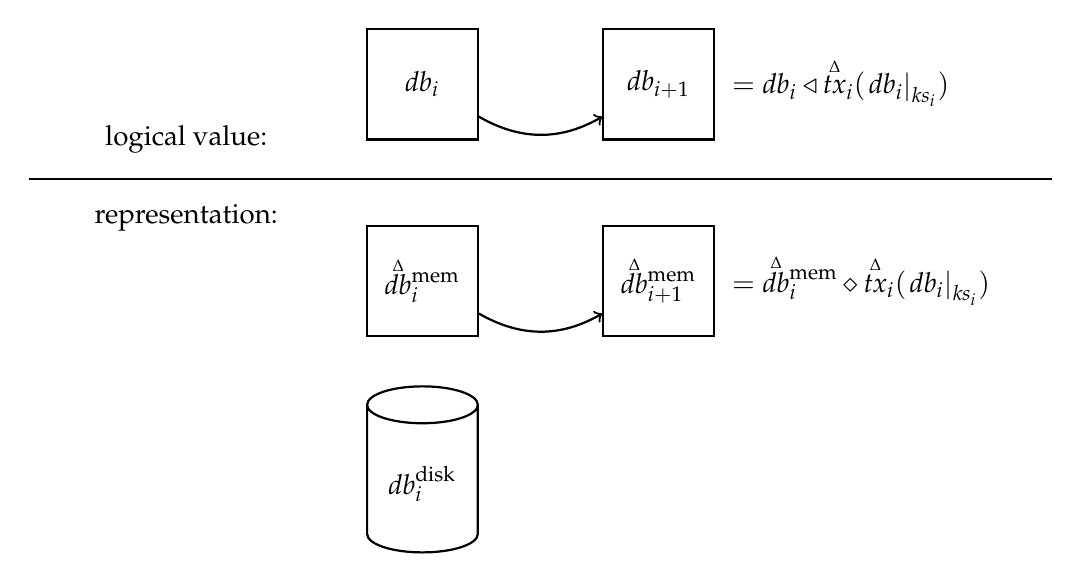
\begin{tikzpicture}
\begin{scope}[thick]

  % disk icon
  \node[cylinder, aspect=2, rotate=90, draw, minimum height=60pt, minimum width=40pt]
        at (0,-25pt) {};
  \draw (0, -25pt) node {$\mathit{db}^{\mathrm{disk}}_i$};

  % in memory
  \begin{scope}[rectangle, minimum height=40pt, minimum width=40pt]
  \node[draw] (mem1) at (0pt,1cm+20pt) {$\deltavar{\mathit{db}}^{\mathrm{mem}}_i$};
  \node[draw] (mem2) at (3cm,1cm+20pt) {$\deltavar{\mathit{db}}^{\mathrm{mem}}_{i+1}$};
  \path[->] (mem1) edge [bend right] (mem2);
  \end{scope}
  \draw (3.8,1cm+20pt) node[anchor=west] {$ = \deltavar{\mathit{db}}^{\mathrm{mem}}_i
                  \diamond \deltavar{\mathit{tx}}_i(\restrict{\mathit{db}_i}{\mathit{ks}_i})$};

  % dividing line
  \draw (-5,3) -- (8,3);
  \draw (-3,3.5) node {logical value:};
  \draw (-3,2.5) node {representation:};

  % logical value
  \begin{scope}[rectangle, minimum height=40pt, minimum width=40pt]
  \node[draw] (logic1) at (0,3.5cm+20pt) {$\mathit{db}_i$};
  \node[draw] (logic2) at (3,3.5cm+20pt) {$\mathit{db}_{i+1}$};
  \path[->] (logic1) edge [bend right] (logic2);
  \end{scope}
  \draw (3.8,3.5cm+20pt) node[anchor=west] {$ = \mathit{db}_i \triangleleft \deltavar{\mathit{tx}}_i(\restrict{\mathit{db}_i}{\mathit{ks}_i})$};
\end{scope}
\end{tikzpicture}
\end{center}
Notice that we have applied the transaction exclusively to the in-memory part,
without changing the on-disk part. Obviously, we cannot do this indefinitely or
the size of the in-memory part will grow without bound.

\subsubsection{Flushing changes to disk}
In this approach, we must flush changes to disk from time to time. Let us see
how that might work. Of course, flushing is not supposed to change the logical
value of the database. It is just supposed to shuffle data from the in-memory
part to the on-disk part. Suppose we start from a state
\[
\mathit{db} = \mathit{db}^{\mathrm{disk}}
      \triangleleft \deltavar{\mathit{db}}^{\mathrm{mem}}
\]
Suppose further that the in-memory part consists of the composition of (at
least) two sets of changes.
\[
\deltavar{\mathit{db}}^{\mathrm{mem}} = \deltavar{\mathit{db}}^{\mathrm{mem}}_a \diamond \deltavar{\mathit{db}}^{\mathrm{mem}}_b
\]
This will be a typical situation since, as we saw above, applying each
transaction gives an extra composition of changes. The idea is that the first
part will be flushed to disk and the second part will remain in memory. We have
a lot of choice here. We can split this in any way we like, in particular at
any boundary between changes from transactions. For example, we could choose to flush
everything to disk by picking
$\deltavar{\mathit{db}}^{\mathrm{mem}}_b = \mathbf{0}$,
but we can also choose to flush just a prefix of changes.

Doing the flush is another straightforward application of
\cref{eq:apply-compose}, but in the opposite direction.
\begin{align*}
       & \mathit{db} = \mathit{db}^{\mathrm{disk}}
         \triangleleft \left( \deltavar{\mathit{db}}^{\mathrm{mem}}_a \diamond \deltavar{\mathit{db}}^{\mathrm{mem}}_b \right)
\\
\equiv & \\
       & \mathit{db} = \left(\mathit{db}^{\mathrm{disk}}
      \triangleleft \deltavar{\mathit{db}}^{\mathrm{mem}}_a \right) \triangleleft \deltavar{\mathit{db}}^{\mathrm{mem}}_b
\end{align*}
We can interpret the application of changes
$\mathit{db}^{\mathrm{disk}} \triangleleft \deltavar{\mathit{db}}^{\mathrm{mem}}_a$
as performing the writes to the on-disk database.
Here is the same in pictorial style:
\begin{center}
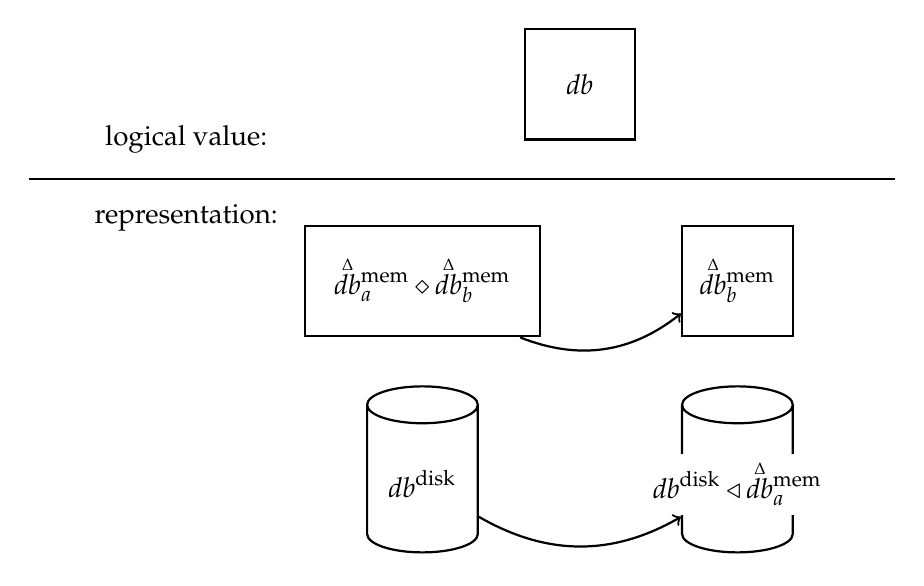
\begin{tikzpicture}
\begin{scope}[thick]

  % disk icon
  \begin{scope}[]
  \node[cylinder, aspect=2, rotate=90, draw, minimum height=60pt, minimum width=40pt]
       (disk1) at (0,-25pt) {};
  \draw (0, -25pt) node {$\mathit{db}^{\mathrm{disk}}$};
  \end{scope}

  \begin{scope}[xshift=4cm]
  \node[cylinder, aspect=2, rotate=90, draw, minimum height=60pt, minimum width=40pt]
       (disk2) at (0,-25pt) {};
  \draw (0, -25pt) node[fill=white] {$\mathit{db}^{\mathrm{disk}} \triangleleft \deltavar{\mathit{db}}^{\mathrm{mem}}_a$};
  \end{scope}
  \path[->] (disk1) edge [bend right] (disk2);

  % in memory
  \begin{scope}[rectangle, minimum height=40pt, minimum width=40pt]
  \node[draw, minimum width=85pt] (mem1) at (0,1cm+20pt)
              {$\deltavar{\mathit{db}}^{\mathrm{mem}}_a \diamond
                 \deltavar{\mathit{db}}^{\mathrm{mem}}_b$};

  \node[draw] (mem2) at (4cm,1cm+20pt)
              {$\deltavar{\mathit{db}}^{\mathrm{mem}}_b$};
  \path[->] (mem1) edge [bend right] (mem2);

  % dividing line
  \draw (-5,3) -- (6,3);
  \draw (-3,3.5) node {logical value:};
  \draw (-3,2.5) node {representation:};

  % logical value
  \node[draw] at (2cm,3.5cm+20pt) {$\mathit{db}$};
  \end{scope}
\end{scope}
\end{tikzpicture}
\end{center}

\subsubsection{Performing reads}

A detail we glossed over above is how we perform reads in this
representation. We said above (in \cref{performing-transactions}) that
\[
\mathit{db}_{i+1} = \mathit{db}_i \triangleleft \deltavar{\mathit{tx}}_i\left(\restrict{\mathit{db}_i}{\mathit{ks}_i}\right)
\]
but we glossed over how we obtain the read set
$\restrict{\mathit{db}_i}{\mathit{ks}_i}$. In the context of the hybrid
in-memory / on-disk database representation, we are interested in how this
corresponds to operations involving the on-disk and in-memory parts. So let us
look at the read set in the context of using it with the transaction function
and rewrite it into a more useful form
\begin{align*}
       & \deltavar{\mathit{tx}}_i\left(\restrict{\mathit{db}_i}{\mathit{ks}_i}\right)
\\
\equiv & \quad \text{\{by \cref{eq:hybrid-db}, expanding the definition ~$\mathit{db}_i = \mathit{db}^{\mathrm{disk}}_i \triangleleft \deltavar{\mathit{db}}^{\mathrm{mem}}_i$\}}
\\
       & \deltavar{\mathit{tx}}_i\left(\restrict{\left(\mathit{db}^{\mathrm{disk}}_i \triangleleft \deltavar{\mathit{db}}^{\mathrm{mem}}_i\right)}{\mathit{ks}_i}\right)
\\
\equiv & \quad \text{\{by \cref{eq:restriction_corollary}, the corollary that ~$\deltavar{\mathit{tx}}_i\left(\restrict{\left(\mathit{db} \triangleleft \deltavar{\mathit{db}}\right)}{\mathit{ks}}\right)
=
  \deltavar{\mathit{tx}}_i\left(\restrict{\mathit{db}}{\mathit{ks}} \triangleleft \deltavar{\mathit{db}}\right)$\}}
\\
       & \deltavar{\mathit{tx}}_i\left(\restrict{\mathit{db}^{\mathrm{disk}}_i}{\mathit{ks}_i} \triangleleft \deltavar{\mathit{db}}^{\mathrm{mem}}_i\right)
\end{align*}
This is a very useful result. The value $\restrict{\mathit{db}^{\mathrm{disk}}_i}{\mathit{ks}_i}$
corresponds to performing a set of reads from the on-disk part of the database.
Notice that we needed the context of using the read set in the transaction to
apply \cref{eq:restriction_corollary}. The intuition is that pushing the
domain restriction inside of applying the in-memory changes could increase the
size of the read set, but the transaction is guaranteed not to look at anything
outside the $\mathit{ks}_i$ subset.

\begin{center}
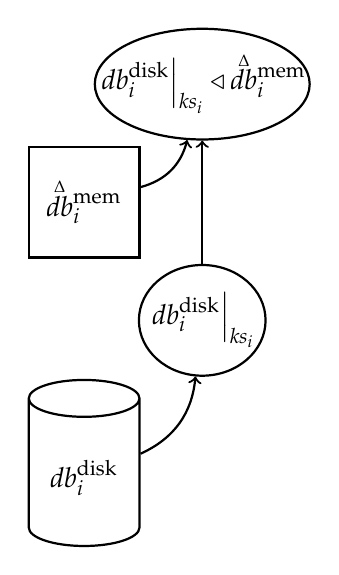
\begin{tikzpicture}
\begin{scope}[thick, minimum width=40pt, minimum height=40pt]

  % disk icon
  \node[cylinder, aspect=2, rotate=90, draw, minimum height=60pt] (disk)
        at (0,-2cm) {};
  \draw (0, -2cm) node {$\mathit{db}^{\mathrm{disk}}_i$};

  % in memory
  \node[rectangle, draw] (mem) at (0,1.5) {$\deltavar{\mathit{db}}^{\mathrm{mem}}_i$};

  % reads
  \node[ellipse, draw, inner sep=-3pt] (read) at (1.5,0)
       {$\restrict{\mathit{db}^{\mathrm{disk}}_i}{\mathit{ks}_i}$};
  \node[ellipse, draw, inner sep=-10pt] (readset) at (1.5,3)
       {$\restrict{\mathit{db}^{\mathrm{disk}}_i}{\mathit{ks}_i}
         \triangleleft \deltavar{\mathit{db}}^{\mathrm{mem}}_i$};

  \draw[->] (disk) edge [bend right] (read);
  \draw[->] (read) edge              (readset);
  \draw[->] (mem)  edge[bend right]  (readset);

\end{scope}
\end{tikzpicture}
\end{center}

Overall, we see that we can perform reads on the hybrid representation simply
by performing the reads on the on-disk part and then applying the in-memory
differences to the result. This is something that can be implemented in a
relatively simple and efficient way.

\subsection{Multiple logical database states}
\label{multiple-logical-database-states}

This model covers the full idea from \cref{access-to-multiple-logical-ledger-states},
in which we want to maintain and have efficient access to many logical values of
a database at once. In particular, we want to model having a single on-disk state
at once and a whole series of in-memory differences, giving us a series of
logical database values.

\begin{center}
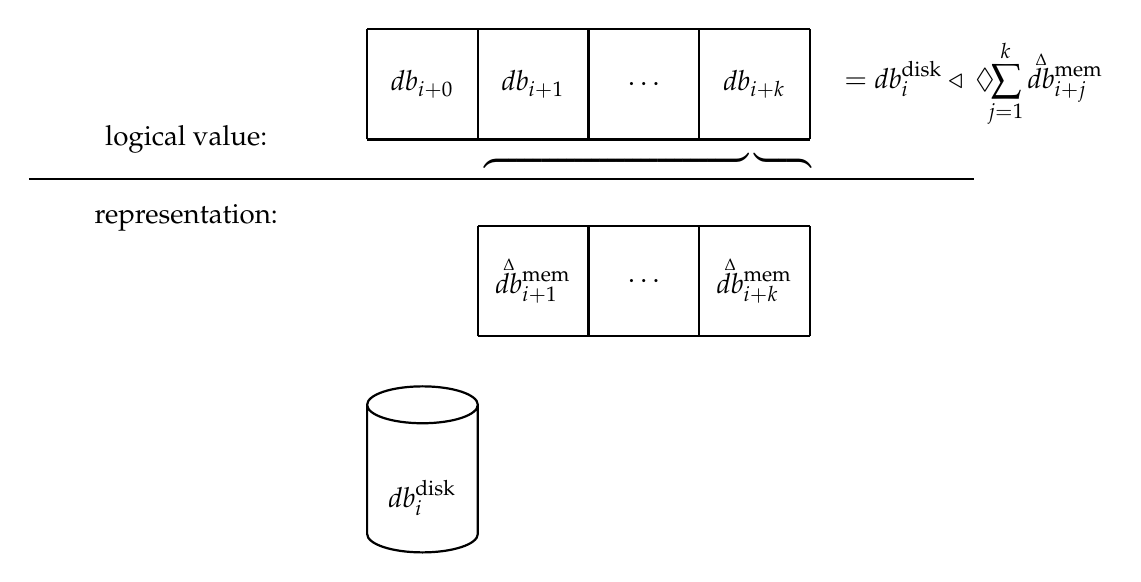
\begin{tikzpicture}[state/.style={circle, draw=black}]
\begin{scope}[thick]

  % disk icon
  \node[cylinder, aspect=2, rotate=90, draw, minimum height=60pt, minimum width=40pt]
        at (0,-25pt) {};
  \draw (0, -30pt) node {$\mathit{db}^{\mathrm{disk}}_i$};

  \begin{scope}[yshift=1cm, xshift=40pt]
  \draw[step=40pt,xshift=-20pt] (0,0) grid (120pt,40pt);
  \draw (0pt,  20pt) node {$\deltavar{\mathit{db}}^{\mathrm{mem}}_{i+1}$};
  \draw (40pt, 20pt) node {$\ldots$};
  \draw (80pt, 20pt) node {$\deltavar{\mathit{db}}^{\mathrm{mem}}_{i+k}$};
  \end{scope}

  % dividing line
  \draw (-5,3) -- (7,3);
  \draw (-3,3.5) node {logical value:};
  \draw (-3,2.5) node {representation:};

  % logical value
  \begin{scope}[yshift=3.5cm]
  \draw[step=40pt,xshift=-20pt] (0,0) grid (160pt,40pt);
  \draw (0,     20pt) node {$\mathit{db}_{i+0}$};
  \draw (40pt,  20pt) node {$\mathit{db}_{i+1}$};
  \draw (80pt,  20pt) node {$\ldots$};
  \draw (120pt, 20pt) node {$\mathit{db}_{i+k}$};
  \end{scope}

  \node [above delimiter=\rmoustache,
         xshift=70pt,yshift=2.9cm, minimum width=100pt] {};
  \node [above delimiter=\lmoustache,
         xshift=130pt,yshift=2.9cm, minimum width=20pt] {};

  \draw (7,3.5cm+20pt) node
        {$= \mathit{db}^{\mathrm{disk}}_i \triangleleft ~
            \displaystyle\Diamond\hspace{-4pt}\sum_{j=1}^k{\deltavar{\mathit{db}}^{\mathrm{mem}}_{i+j}}$};

\end{scope}
\end{tikzpicture}
\end{center}
As depicted above, the representation consists of a single disk
state and a series of in-memory differences. Each difference is the individual
difference from performing a transaction. That is, we keep each difference and
do not compose them together prematurely. Each logical database value is
the value of the on-disk state with the monoidal composition of the appropriate
changes applied on top. That is, for the k\textsuperscript{th} database value
beyond the on-disk state we have
\[
\mathit{db}_{i+k}
= \mathit{db}^{\mathrm{disk}}_i \triangleleft ~
            \displaystyle\Diamond\hspace{-4pt}\sum_{j=0}^k{\deltavar{\mathit{db}}^{\mathrm{mem}}_{i+j}}
\]
which of course for the zero case is simply
\[
\mathit{db}_{i+0}
= \mathit{db}^{\mathrm{disk}}_i
\]
Although we are interested in the compositions of differences, we must keep the
individual differences. The reason is that, when we do flush changes to disk, we
need to discard the oldest in-memory differences, which entails computing new
monoidal compositions of the remaining differences.

One interesting implementation idea to manage both a sequence of $k$ differences
and also the efficient monoidal composition of them is to use a \emph{finger
tree} data structure \citep{fingertree}. A finger tree is parametrised over a
monoidal measure of subsequences. The choice of measure for a subsequence in
this case would be the range of slot numbers and also the composition of the
differences. The slot number range is included to support splitting at slot numbers. We
would rely on splitting to obtain the subsequence of differences for
evaluating a chain fork that starts from a recent point on the chain. Including the other
part of the measure -- the differences -- would mean that the measure of any
sequence or sub-sequence would be the overall monoidal composition of all the
differences in that (sub-)sequence. The finger tree data structure takes care
of efficiently caching the intermediate, monoidal measure values. Finger trees are
already used extensively within the consensus implementation.

There are a few operations we need to be able to perform in this setting:
\begin{enumerate}
\item Perform reads of sets of keys and `forward' the resulting read set
      using the accumulated sequence of differences.
\item Replace any suffix of the sequence of logical database values. This
      corresponds to switching to a fork. The replacement subsequence can
      start anywhere in the sequence, and the replacement subsequence can have any length.
      The very common special case
      is to append to the end of the sequence of logical database values.
      This corresponds to adding a block to the end of the chain, or adding
      more transactions to a mempool.
\item Flush changes to disk. We need to be able to take some of the oldest
      changes and apply them to the on-disk store.
\end{enumerate}
These operations are straightforward generalisations of the operations we have
already seen in \cref{sec:hybrid-on-disk-in-memory-db}. The first two are about
constructing new logical database values by making new in-memory differences.
In this representation, it is achieved by simply appending or replacing a suffix of a
sequence of changes. The flushing to disk is a straightforward instance of the
flush operation from \cref{sec:hybrid-on-disk-in-memory-db} where we choose
a point in the sequence that splits the differences we wish to flush from the
remaining sequence of differences that should be kept in memory. The value that we apply to the on-disk state
is the monoidal composition of the sequence of differences we wish to flush.

\subsection{Change-based pipelined databases}

Here is where things start to get interesting and tricky. As discussed in
\cref{enabling-pipelining}, we wish to pipeline reads from disk to provide the
opportunity to use parallel I/O. Providing this opportunity is not something
that we can hide away in some low-level I/O layer: it will have to be explicit
in how we manage the logical state of the database. So, the purpose of this
model is to provide a reasonable correspondence to an implementation that could use
pipelined reads. We will also want to show that it is nevertheless
mathematically equivalent to the simple model.

The goal with the pipelining of I/O reads is to initiate the I/O operations
early such that the results are already available in memory by the time they are
needed later. This allows the I/O to be overlapped with computation, and it
also allows a substantial number of I/O operations to be in progress at once,
which is what provides the opportunity to use parallel I/O.

Recall the sequential pattern from \cref{change-based-databases} where the
reads and transactions are based on the immediately preceding database value.
\begin{center}
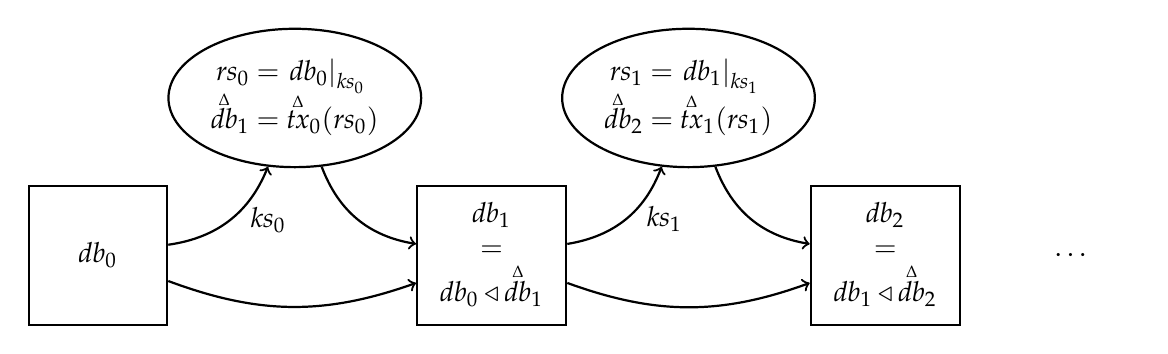
\begin{tikzpicture}
\begin{scope}[thick, rectangle, minimum width=50pt, minimum height=50pt]
  \node[draw] (db0)           {$\mathit{db}_0$};
  \node[draw] (db1) at (5,0)  {$\eqabove{\mathit{db}_1}{\mathit{db}_0 \triangleleft \deltavar{\mathit{db}}_1}$};
  \node[draw] (db2) at (10,0) {$\eqabove{\mathit{db}_2}{\mathit{db}_1 \triangleleft \deltavar{\mathit{db}}_2}$};
  \node[right=0.5cm of db2] {$\ldots$};

  % read sets and transaction differences
  \node[ellipse, draw, inner sep=-3pt] (rs0) at (2.5cm, 2cm)
       {$\begin{array}{r@{~=~}l}
           \mathit{rs}_0 & \restrict{\mathit{db}_0}{\mathit{ks}_0} \\
           \deltavar{\mathit{db}}_1 & \deltavar{\mathit{tx}}_0(\mathit{rs}_0)
         \end{array}$};
  \node[ellipse, draw, inner sep=-3pt] (rs1) at (7.5cm, 2cm)
       {$\begin{array}{r@{~=~}l}
           \mathit{rs}_1 & \restrict{\mathit{db}_1}{\mathit{ks}_1} \\
           \deltavar{\mathit{db}}_2 & \deltavar{\mathit{tx}}_1(\mathit{rs}_1)
         \end{array}$};

  \path[->] (db0) edge [bend right] node[right=-0.4] {$\mathit{ks}_0$} (rs0);
  \path[->] (db1) edge [bend right] node[right=-0.4] {$\mathit{ks}_1$} (rs1);

  \path[->] (rs0) edge [bend right] (db1);
  \path[->] (rs1) edge [bend right] (db2);

  \path[->] (db0) edge [bend right=20] (db1);
  \path[->] (db1) edge [bend right=20] (db2);
\end{scope}
\end{tikzpicture}
\end{center}
The difficulty with initiating the reads early is that the state of the
database in which we initiated the reads is not the same state as the one in
which we use the read results to perform a transaction. For example, if we
na\"ively started the reads for $\mathit{ks}_1$ from $\mathit{db}_0$, expecting
to use it later with $\deltavar{\mathit{tx}}_1$, then any updates applied by
$\deltavar{\mathit{tx}}_0$ in $\mathit{db}_1$ that might affect the read set
would be lost and we would get the wrong result.
\begin{center}
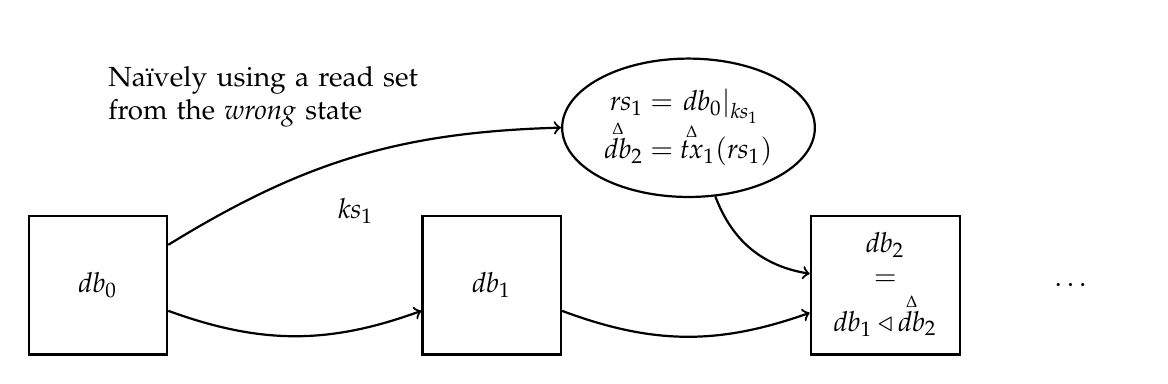
\begin{tikzpicture}
\begin{scope}[thick, rectangle, minimum width=50pt, minimum height=50pt]
  \node[draw] (db0)           {$\mathit{db}_0$};
  \node[draw] (db1) at (5,0)  {$\mathit{db}_1$};
  \node[draw] (db2) at (10,0) {$\eqabove{\mathit{db}_2}{\mathit{db}_1 \triangleleft \deltavar{\mathit{db}}_2}$};
  \node[right=0.5cm of db2] {$\ldots$};

  % read sets and transaction differences
  \node[ellipse, draw, inner sep=-3pt] (rs1) at (7.5cm, 2cm)
       {$\begin{array}{r@{~=~}l}
           \mathit{rs}_1 & \restrict{\mathit{db}_0}{\mathit{ks}_1} \\
           \deltavar{\mathit{db}}_2 & \deltavar{\mathit{tx}}_1(\mathit{rs}_1)
         \end{array}$};

  \path[->] (db0) edge [bend left=15] node[below=-0.2] {$\mathit{ks}_1$} (rs1);
  \node[above=1.5cm of db0, anchor=west, text width=4.5cm]
       {Na\"ively using a read set from the \emph{wrong} state};

  \path[->] (rs1) edge [bend right] (db2);
  \path[->] (db0) edge [bend right=20] (db1);
  \path[->] (db1) edge [bend right=20] (db2);
\end{scope}
\end{tikzpicture}
\end{center}
Of course, pipelining is only acceptable if we can find some way to make it
semantically equivalent to the sequential version. The trick to do so is to
adjust the result of the reads so that it is \emph{as if} they had been
performed against the right state of the database.

Notice in the sequential example above that $\mathit{db}_1$ is $\mathit{db}_0$
with some changes applied to it, and a read set from $\mathit{db}_0$ is simply a
subset of $\mathit{db}_0$, so if we apply the same changes to the read set, then
that should be the same as if we had performed the read from $\mathit{db}_1$ in
the first place. In pictorial form, it would look like the following, with the
reads of $\mathit{ks}_1$ intended to be used with $\deltavar{\mathit{tx}}_1$
being started against $\mathit{db}_0$, and then later adjusted by applying the
changes from $\deltavar{\mathit{tx}}_0$.
\begin{center}
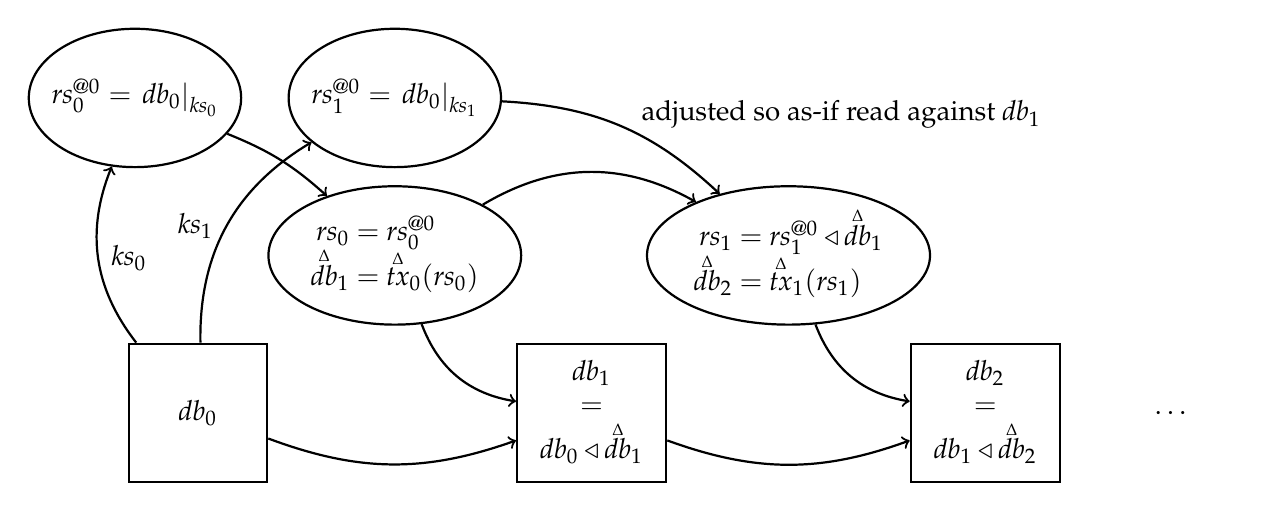
\begin{tikzpicture}
\begin{scope}[thick, rectangle, minimum width=50pt, minimum height=50pt]
  \node[draw] (db0) {$\mathit{db}_0$};
  \node[draw] (db1) at (5cm,0)
       {$\eqabove{\mathit{db}_1}
                 {\mathit{db}_0 \triangleleft \deltavar{\mathit{db}}_1}$};
  \node[draw] (db2) at (10cm,0)
       {$\eqabove{\mathit{db}_2}
                 {\mathit{db}_1 \triangleleft \deltavar{\mathit{db}}_2}$};
  \node[right=0.5cm of db2] {$\ldots$};

  % read sets and transaction differences
  \node[ellipse, draw, inner sep=-3pt] (rs0) at (2.5cm, 2cm)
       {$\begin{array}{r@{~=~}l}
           \mathit{rs}_0 & \mathit{rs}^{@0}_{0} \\
           \deltavar{\mathit{db}}_1 & \deltavar{\mathit{tx}}_0(\mathit{rs}_0)
         \end{array}$};
  \node[ellipse, draw, inner sep=-3pt] (rs1) at (7.5cm, 2cm)
       {$\begin{array}{r@{~=~}l}
           \mathit{rs}_1 & \mathit{rs}^{@0}_{1} \triangleleft \deltavar{\mathit{db}}_1 \\
           \deltavar{\mathit{db}}_2 & \deltavar{\mathit{tx}}_1(\mathit{rs}_1)
         \end{array}$};

  \node[ellipse, draw, inner sep=-3pt] (rs0_0) at (-0.8, 4cm)
       {$\mathit{rs}^{@0}_{0} = \restrict{\mathit{db}_0}{\mathit{ks}_0}$};
  \node[ellipse, draw, inner sep=-3pt] (rs1_0) at (2.5, 4cm)
       {$\mathit{rs}^{@0}_{1} = \restrict{\mathit{db}_0}{\mathit{ks}_1}$};


  \path[->] (db0) edge [bend left] node[right=-0.5] {$\mathit{ks}_0$} (rs0_0);
  \path[->] (db0) edge [bend left] node[left=-0.5]  {$\mathit{ks}_1$} (rs1_0);

  \path[->] (rs0) edge [bend right] (db1);
  \path[->] (rs1) edge [bend right] (db2);

  \path[->] (rs0_0) edge [bend left=10] (rs0);
  \path[->] (rs1_0) edge [bend left=20]
                    node [above right=0.2, anchor=west]
                    {adjusted so as-if read against $\mathit{db}_1$}
            (rs1);
  \path[->] (rs0)   edge [bend left=30] (rs1);

  \path[->] (db0) edge [bend right=20] (db1);
  \path[->] (db1) edge [bend right=20] (db2);
\end{scope}
\end{tikzpicture}
\end{center}
We can now extend this example so that after the initial step (where we
perform two reads from $\mathit{db}_0$ to get things going) we always
initiate a read to be used by the next-but-one transaction. This gives us
pipelining of depth one. This pattern could be extended indefinitely, and
greater (or variable) depth pipelining could be used.
\begin{center}
\resizebox{\textwidth}{!}{%
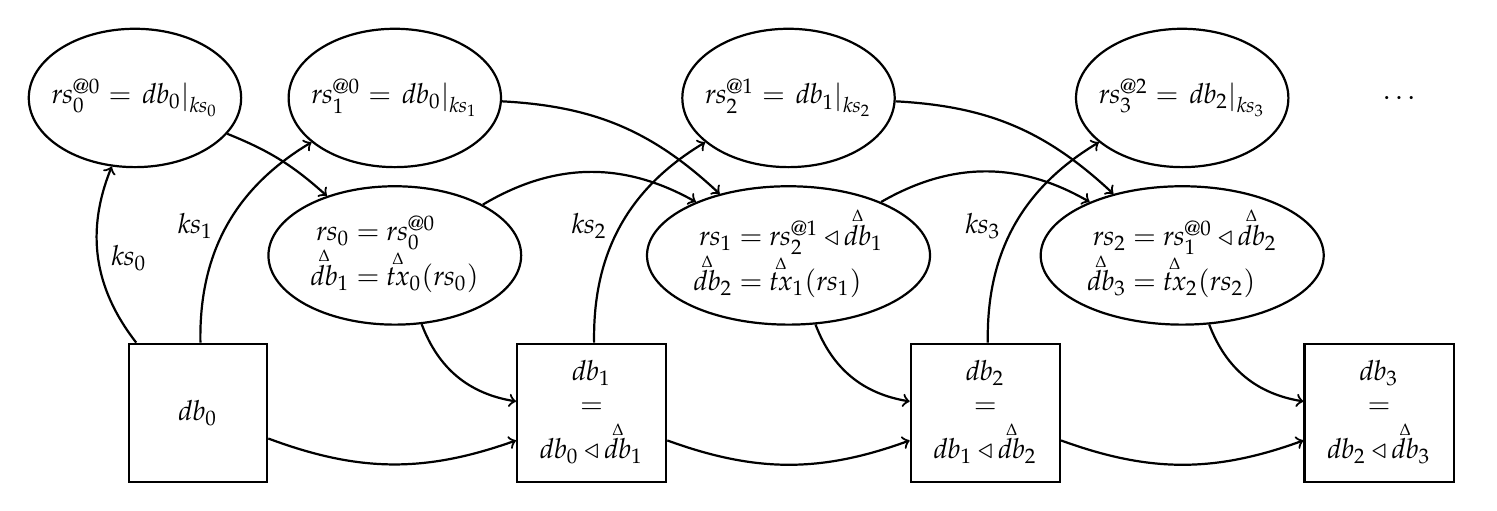
\begin{tikzpicture}
\begin{scope}[thick, rectangle, minimum width=50pt, minimum height=50pt]
  \node[draw] (db0) {$\mathit{db}_0$};
  \node[draw] (db1) at (5cm,0)
       {$\eqabove{\mathit{db}_1}
                 {\mathit{db}_0 \triangleleft \deltavar{\mathit{db}}_1}$};
  \node[draw] (db2) at (10cm,0)
       {$\eqabove{\mathit{db}_2}
                 {\mathit{db}_1 \triangleleft \deltavar{\mathit{db}}_2}$};
  \node[draw] (db3) at (15cm,0)
       {$\eqabove{\mathit{db}_3}
                 {\mathit{db}_2 \triangleleft \deltavar{\mathit{db}}_3}$};

  % read sets and transaction differences
  \node[ellipse, draw, inner sep=-3pt] (rs0) at (2.5cm, 2cm)
       {$\begin{array}{r@{~=~}l}
           \mathit{rs}_0 & \mathit{rs}^{@0}_{0} \\
           \deltavar{\mathit{db}}_1 & \deltavar{\mathit{tx}}_0(\mathit{rs}_0)
         \end{array}$};
  \node[ellipse, draw, inner sep=-3pt] (rs1) at (7.5cm, 2cm)
       {$\begin{array}{r@{~=~}l}
           \mathit{rs}_1 & \mathit{rs}^{@1}_{2} \triangleleft \deltavar{\mathit{db}}_1 \\
           \deltavar{\mathit{db}}_2 & \deltavar{\mathit{tx}}_1(\mathit{rs}_1)
         \end{array}$};
  \node[ellipse, draw, inner sep=-3pt] (rs2) at (12.5cm, 2cm)
       {$\begin{array}{r@{~=~}l}
           \mathit{rs}_2 & \mathit{rs}^{@0}_{1} \triangleleft \deltavar{\mathit{db}}_2 \\
           \deltavar{\mathit{db}}_3 & \deltavar{\mathit{tx}}_2(\mathit{rs}_2)
         \end{array}$};
  \node[ellipse, draw, inner sep=-3pt] (rs0_0) at (-0.8, 4cm)
       {$\mathit{rs}^{@0}_{0} = \restrict{\mathit{db}_0}{\mathit{ks}_0}$};
  \node[ellipse, draw, inner sep=-3pt] (rs1_0) at (2.5, 4cm)
       {$\mathit{rs}^{@0}_{1} = \restrict{\mathit{db}_0}{\mathit{ks}_1}$};
  \node[ellipse, draw, inner sep=-3pt] (rs2_1) at (7.5, 4cm)
       {$\mathit{rs}^{@1}_{2} = \restrict{\mathit{db}_1}{\mathit{ks}_2}$};
  \node[ellipse, draw, inner sep=-3pt] (rs3_2) at (12.5, 4cm)
       {$\mathit{rs}^{@2}_{3} = \restrict{\mathit{db}_2}{\mathit{ks}_3}$};
  \node[right=0.5cm of rs3_2] {$\ldots$};

  \path[->] (db0) edge [bend left] node[right=-0.5] {$\mathit{ks}_0$} (rs0_0);
  \path[->] (db0) edge [bend left] node[left=-0.5]  {$\mathit{ks}_1$} (rs1_0);
  \path[->] (db1) edge [bend left] node[left=-0.5]  {$\mathit{ks}_2$} (rs2_1);
  \path[->] (db2) edge [bend left] node[left=-0.5]  {$\mathit{ks}_3$} (rs3_2);

  \path[->] (rs0) edge [bend right] (db1);
  \path[->] (rs1) edge [bend right] (db2);
  \path[->] (rs2) edge [bend right] (db3);

  \path[->] (rs0_0) edge [bend left=10] (rs0);
  \path[->] (rs1_0) edge [bend left=20] (rs1);
  \path[->] (rs2_1) edge [bend left=20] (rs2);

  \path[->] (rs0)   edge [bend left=30] (rs1);
  \path[->] (rs1)   edge [bend left=30] (rs2);

  \path[->] (db0) edge [bend right=20] (db1);
  \path[->] (db1) edge [bend right=20] (db2);
  \path[->] (db2) edge [bend right=20] (db3);
\end{scope}
\end{tikzpicture}
}
\begin{equation*}
\begin{array}{c@{\quad}l@{\quad}l@{\quad}l}
    \mathit{db}_1 = \mathit{db}_0 \triangleleft \deltavar{\mathit{db}}_1
  & \mathbf{where} \quad \deltavar{\mathit{db}}_1 = \deltavar{\mathit{tx}}_0(\mathit{rs}_0)
  & \mathbf{and}   \quad \mathit{rs}_0 = \mathit{rs}^{@0}_0
  & \mathbf{and}   \quad \mathit{rs}^{@0}_0 = \restrict{\mathit{db}_0}{\mathit{ks}_0}
\\
    \mathit{db}_2 = \mathit{db}_1 \triangleleft \deltavar{\mathit{db}}_2
  & \mathbf{where} \quad \deltavar{\mathit{db}}_2 = \deltavar{\mathit{tx}}_1(\mathit{rs}_1)
  & \mathbf{and}   \quad \mathit{rs}_1 = \mathit{rs}^{@0}_1 \triangleleft \deltavar{\mathit{db}}_1
  & \mathbf{and}   \quad \mathit{rs}^{@0}_1 = \restrict{\mathit{db}_0}{\mathit{ks}_1}
\\
    \mathit{db}_3 = \mathit{db}_2 \triangleleft \deltavar{\mathit{db}}_3
  & \mathbf{where} \quad \deltavar{\mathit{db}}_3 = \deltavar{\mathit{tx}}_2(\mathit{rs}_2)
  & \mathbf{and}   \quad \mathit{rs}_2 = \mathit{rs}^{@1}_2 \triangleleft \deltavar{\mathit{db}}_2
  & \mathbf{and}   \quad \mathit{rs}^{@1}_2 = \restrict{\mathit{db}_1}{\mathit{ks}_2}
\\
\end{array}
\end{equation*}
\vdots \\
And in general (for $i > 1$)
\begin{equation*}
\begin{array}{c@{~}l@{\quad}l@{\quad}l}
    \mathit{db}_{i+1} = \mathit{db}_i \triangleleft \deltavar{\mathit{db}}_{i+1}
  & \mathbf{where} \quad \deltavar{\mathit{db}}_{i+1} = \deltavar{\mathit{tx}}_i(\mathit{rs}_i)
  & \mathbf{and}   \quad \mathit{rs}_i = \mathit{rs}^{@{i-1}}_i \triangleleft \deltavar{\mathit{db}}_i
  & \mathbf{and}   \quad \mathit{rs}^{@{i-1}}_i = \restrict{\mathit{db}_{i-1}}{\mathit{ks}_i}
\end{array}
\end{equation*}
\end{center}
We need to clarify how exactly this is equivalent to the simple sequential
model. We now have a more interesting recurrence relation than in previous
models, so we argue by induction. Due to the setup step for the pipelining, we
start from $i=1$ rather than $i=0$.
\begin{align*}
       & \mathit{db}_{i+1} = \mathit{db}_i \triangleleft \deltavar{\mathit{db}}_{i+1}
         \quad \mathbf{where} \quad \deltavar{\mathit{db}}_{i+1} = \deltavar{\mathit{tx}}_i(\mathit{rs}_i)
         \quad \mathbf{and} \quad \mathit{rs}_i = \mathit{rs}^{@{i-1}}_i \triangleleft \deltavar{\mathit{db}}_i
         \quad \mathbf{and} \quad \mathit{rs}^{@i-1}_i = \restrict{\mathit{db}_{i-1}}{\mathit{ks}_i}
      \\
\equiv & \quad \text{\{by substitution of $\mathit{rs}_i$ and $\mathit{rs}^{@i-1}_i$ \}}
      \\
       & \mathit{db}_{i+1} = \mathit{db}_i \triangleleft \deltavar{\mathit{db}}_{i+1}
         \quad \mathbf{where} \quad \deltavar{\mathit{db}}_{i+1} = \deltavar{\mathit{tx}}_i\left(\restrict{\mathit{db}_{i-1}}{\mathit{ks}_i} \triangleleft \deltavar{\mathit{db}}_{i}\right)
      \\
\equiv & \quad \text{\{by the domain restriction shifting lemma \cref{eq:restriction_corollary} \}}
      \\
       & \mathit{db}_{i+1} = \mathit{db}_i \triangleleft \deltavar{\mathit{db}}_{i+1}
         \quad \mathbf{where} \quad \deltavar{\mathit{db}}_{i+1} = \deltavar{\mathit{tx}}_i\left(\restrict{\left(\mathit{db}_{i-1} \triangleleft \deltavar{\mathit{db}}_{i}\right)}{\mathit{ks}_i}\right)
      \\
\equiv & \quad \text{\{by induction hypothesis $\mathit{db}_i = \mathit{db}_{i-1} \triangleleft \deltavar{\mathit{db}}_{i}$ \}}
      \\
       & \mathit{db}_{i+1} = \mathit{db}_i \triangleleft \deltavar{\mathit{db}}_{i+1}
         \quad \mathbf{where} \quad \deltavar{\mathit{db}}_{i+1} = \deltavar{\mathit{tx}}_i\left(\restrict{\mathit{db}_i}{\mathit{ks}_i}\right)
      \\
\equiv & \quad \text{\{by substitution of $\deltavar{\mathit{db}}_{i+1}$\}}
      \\
       & \mathit{db}_{i+1} = \mathit{db}_i \triangleleft \deltavar{\mathit{tx}}_i\left(\restrict{\mathit{db}_i}{\mathit{ks}_i}\right)
      \\
\equiv & \quad \text{\{by the restriction property \cref{eq:tx-within-keyset} that
                     $\deltavar{\mathit{tx}}_i\left(\restrict{\mathit{db}}{\mathit{ks}_i}\right) = \deltavar{\mathit{tx}}_i(\mathit{db})$\}}
      \\
       & \mathit{db}_{i+1} = \mathit{db}_i \triangleleft \deltavar{\mathit{tx}}_i(\mathit{db}_i)
      \\
\equiv & \quad \text{\{by the difference function property \cref{eq:diff-fun} that
                     $db \triangleleft \deltavar{\mathit{tx}}(\mathit{db}) = \mathit{tx}(\mathit{db})$\}}
      \\
       & \mathit{db}_{i+1} = \mathit{tx}_i(\mathit{db}_i)
\end{align*}
Which is the same as \cref{eq:sequential-recurrence}: the recurrence for the simple model.

\subsection{Change-based pipelined databases in the hybrid representation}

More generally, the changes we want to apply are all those that occurred between
the database state against which the read was performed and the state in which
the transaction using the read results is to be applied. Thus, we will have to
carefully track and apply the changes from where a read was initiated to where
it is used. If we can do so successfully however, it seems clear that we can
obtain an arbitrary depth of pipelining, at the memory cost of tracking the
intervening changes.

Fortunately, tracking the intervening changes is relatively straightforward to
do using the hybrid representations (from
\cref{sec:hybrid-on-disk-in-memory-db,multiple-logical-database-states}) since
they already keep the recent changes in memory.

The diagram below shows an example of the hybrid representation where several
transactions are performed starting from the same on-disk state. Notice how
all the disk reads are independent and so can be started early. Only the
in-memory adjustments to read sets prior to
processing transactions is still sequential.
\begin{center}
\resizebox{\textwidth}{!}{%
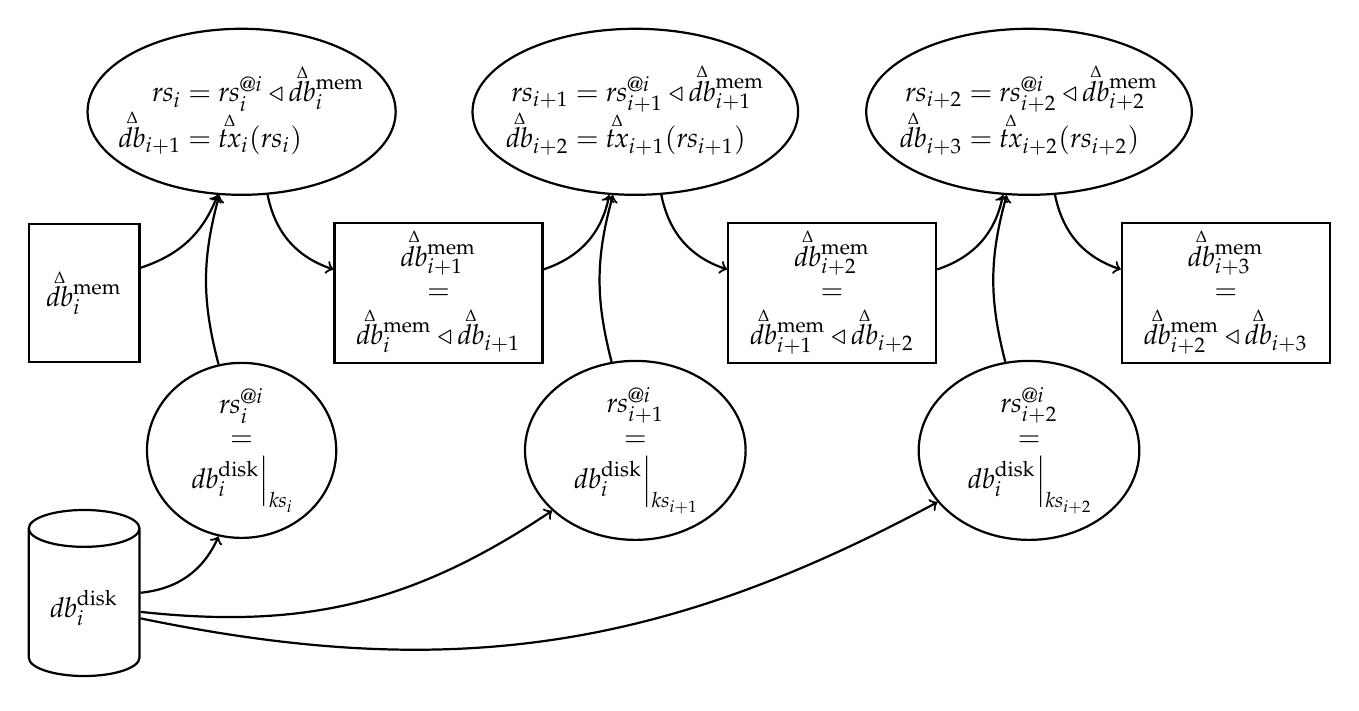
\begin{tikzpicture}
\begin{scope}[thick, minimum height=50pt, minimum width=40pt]

  \node[cylinder, aspect=2, rotate=90, draw, minimum height=60pt]
       (disk) at (0.5,-2.5cm) {};
  \draw (0.5, -2.5cm) node {$\mathit{db}^{\mathrm{disk}}_i$};

  % in mem boxes
  \begin{scope}[inner sep=3pt]
  \node[rectangle, draw] (mem0) at (0.5,   1.5)
       {$\deltavar{\mathit{db}}^{\mathrm{mem}}_i$};
  \node[rectangle, draw] (mem1) at (5cm, 1.5)
       {$\eqabove{\deltavar{\mathit{db}}^{\mathrm{mem}}_{i+1}}
                 {\deltavar{\mathit{db}}^{\mathrm{mem}}_{i} \triangleleft \deltavar{\mathit{db}}_{i+1}}$};
  \node[rectangle, draw] (mem2) at (10cm,1.5)
       {$\eqabove{\deltavar{\mathit{db}}^{\mathrm{mem}}_{i+2}}
                 {\deltavar{\mathit{db}}^{\mathrm{mem}}_{i+1} \triangleleft \deltavar{\mathit{db}}_{i+2}}$};
  \node[rectangle, draw] (mem3) at (15cm,1.5)
       {$\eqabove{\deltavar{\mathit{db}}^{\mathrm{mem}}_{i+3}}
                 {\deltavar{\mathit{db}}^{\mathrm{mem}}_{i+2} \triangleleft \deltavar{\mathit{db}}_{i+3}}$};
  \end{scope}

  % disk reads
  \begin{scope}[inner sep=0pt]
  \node[ellipse, draw] (diskread0) at (2.5cm,-0.5cm)
       {$\eqabove{\mathit{rs}^{@i}_{i}}
                 {\restrict{\mathit{db}^{\mathrm{disk}}_i}{\mathit{ks}_i}}$};

  \node[ellipse, draw] (diskread1) at (7.5cm,-0.5cm)
       {$\eqabove{\mathit{rs}^{@i}_{i+1}}
                 {\restrict{\mathit{db}^{\mathrm{disk}}_i}{\mathit{ks}_{i+1}}}$};

  \node[ellipse, draw] (diskread2) at (12.5cm,-0.5cm)
       {$\eqabove{\mathit{rs}^{@i}_{i+2}}
                 {\restrict{\mathit{db}^{\mathrm{disk}}_i}{\mathit{ks}_{i+2}}}$};
  \end{scope}

  % logical reads and transaction differences
  \begin{scope}[minimum height=60pt, inner sep=-10pt]
  \node[ellipse, draw] (readset1) at (2.5,3.8)
       {$\begin{array}{r@{~=~}l}
           \mathit{rs}_{i} & \mathit{rs}^{@i}_{i} \triangleleft \deltavar{\mathit{db}}^{\mathrm{mem}}_i \\
           \deltavar{\mathit{db}}_{i+1} & \deltavar{\mathit{tx}}_i(\mathit{rs}_i)
         \end{array}$};
  \node[ellipse, draw] (readset2) at (7.5,3.8)
       {$\begin{array}{r@{~=~}l}
          \mathit{rs}_{i+1} & \mathit{rs}^{@i}_{i+1} \triangleleft \deltavar{\mathit{db}}^{\mathrm{mem}}_{i+1} \\
           \deltavar{\mathit{db}}_{i+2} & \deltavar{\mathit{tx}}_{i+1}(\mathit{rs}_{i+1})
         \end{array}$};
  \node[ellipse, draw] (readset3) at (12.5,3.8)
       {$\begin{array}{r@{~=~}l}
          \mathit{rs}_{i+2} & \mathit{rs}^{@i}_{i+2} \triangleleft \deltavar{\mathit{db}}^{\mathrm{mem}}_{i+2} \\
           \deltavar{\mathit{db}}_{i+3} & \deltavar{\mathit{tx}}_{i+2}(\mathit{rs}_{i+2})
         \end{array}$};
  \end{scope}

  % lines reads
  \path[->] (disk) edge [bend right=30] (diskread0);
  \path[->] (disk) edge [bend right=20] (diskread1);
  \path[->] (disk) edge [bend right=20] (diskread2);

  \path[->] (diskread0) edge [bend left=15] (readset1);
  \path[->] (mem0)      edge [bend right=25](readset1);
  \path[->] (readset1)  edge [bend right]   (mem1);

  \path[->] (diskread1) edge [bend left=15] (readset2);
  \path[->] (mem1)      edge [bend right]   (readset2);
  \path[->] (readset2)  edge [bend right]   (mem2);

  \path[->] (diskread2) edge [bend left=15] (readset3);
  \path[->] (mem2)      edge [bend right]   (readset3);
  \path[->] (readset3)  edge [bend right]   (mem3);
\end{scope}
\end{tikzpicture}
}
\end{center}
This example does not include flushing changes to disk, which does also have to
be done eventually. Doing so only marginally complicates the scheme. It involves
keeping in memory the changes between when a read was initiated and when it is
used -- even if some older changes have been flushed to disk in the
meantime.

\addcontentsline{toc}{section}{References}
\bibliographystyle{plainnat}
\bibliography{utxo-db}

\end{document}